\documentclass[sigplan,review,anonymous]{acmart}\settopmatter{printfolios=true,printccs=false,printacmref=false}


\acmConference[SPAA'20]{ACM Symposium on Parallelism in Algorithms and Architectures}{July 14--17, 2020}{Philadelphia, PA, USA} \acmYear{2020}
\acmISBN{} % \acmISBN{978-x-xxxx-xxxx-x/YY/MM}
\acmDOI{} % \acmDOI{10.1145/nnnnnnn.nnnnnnn}
\startPage{1}
\begin{CCSXML}
<ccs2012>
<concept>
<concept_id>10010147</concept_id>
<concept_desc>Computing methodologies</concept_desc>
<concept_significance>500</concept_significance>
</concept>
<concept>
<concept_id>10010147.10010169</concept_id>
<concept_desc>Computing methodologies~Parallel computing methodologies</concept_desc>
<concept_significance>500</concept_significance>
</concept>
<concept>
<concept_id>10010147.10010169.10010170</concept_id>
<concept_desc>Computing methodologies~Parallel algorithms</concept_desc>
<concept_significance>500</concept_significance>
</concept>
<concept>
<concept_id>10010147.10010169.10010170.10010174</concept_id>
<concept_desc>Computing methodologies~Massively parallel algorithms</concept_desc>
<concept_significance>500</concept_significance>
</concept>
</ccs2012>
\end{CCSXML}

\ccsdesc[500]{Computing methodologies}
\ccsdesc[500]{Computing methodologies~Parallel computing methodologies}
\ccsdesc[500]{Computing methodologies~Parallel algorithms}
\ccsdesc[500]{Computing methodologies~Massively parallel algorithms}%% Copyright information
%% Supplied to authors (based on authors' rights management selection;
%% see authors.acm.org) by publisher for camera-ready submission;
%% use 'none' for review submission.
\setcopyright{none}
%\setcopyright{acmcopyright}
%\setcopyright{acmlicensed}
%\setcopyright{rightsretained}
%\copyrightyear{2018}           %% If different from \acmYear

%% Bibliography style
\bibliographystyle{ACM-Reference-Format}
%% Citation style
%\citestyle{acmauthoryear}  %% For author/year citations
%\citestyle{acmnumeric}     %% For numeric citations
%\setcitestyle{nosort}      %% With 'acmnumeric', to disable automatic
                            %% sorting of references within a single citation;
                            %% e.g., \cite{Smith99,Carpenter05,Baker12}
                            %% rendered as [14,5,2] rather than [2,5,14].
%\setcitesyle{nocompress}   %% With 'acmnumeric', to disable automatic
                            %% compression of sequential references within a
                            %% single citation;
                            %% e.g., \cite{Baker12,Baker14,Baker16}
                            %% rendered as [2,3,4] rather than [2-4].


%%%%%%%%%%%%%%%%%%%%%%%%%%%%%%%%%%%%%%%%%%%%%%%%%%%%%%%%%%%%%%%%%%%%%%
%% Note: Authors migrating a paper from traditional SIGPLAN
%% proceedings format to PACMPL format must update the
%% '\documentclass' and topmatter commands above; see
%% 'acmart-pacmpl-template.tex'.
%%%%%%%%%%%%%%%%%%%%%%%%%%%%%%%%%%%%%%%%%%%%%%%%%%%%%%%%%%%%%%%%%%%%%%



\usepackage{booktabs}
\usepackage{subcaption}
\usepackage{listings}
\usepackage{graphicx}
\usepackage[ruled,linesnumbered]{algorithm2e}
\usepackage{url}
\usepackage{enumerate}
\usepackage{amsmath}
\usepackage{multirow}
\usepackage{makecell,rotating}
\usepackage{color, colortbl}

\newcommand\FIXME[1]{\textcolor{red}{FIX:}\textcolor{red}{#1}}


\begin{document}
\title{Optimizing GPU Memory Transactions for Convolution Operations}

\author{Weizhe Zhang}
\affiliation{
  \department{Computer Science and Technology}
  \institution{Harbin Institute of Technology}
  \country{China}
}
\email{wzzhang@hit.edu.cn}

\author{Gangzhao Lu}
\affiliation{
  \department{Computer Science and Technology}              %% \department is recommended
  \institution{Harbin Institute of Technology}            %% \institution is required
  \country{China}                    %% \country is recommended
}
\email{lugangzhao@hit.edu.cn}

\author{Zheng Wang}
\affiliation{
  \department{School of Computing}              %% \department is recommended
  \institution{University of Leeds}            %% \institution is required
  \country{U. K.}                    %% \country is recommended
} \email{zwang5@leeds.ac.uk}

\begin{abstract}
Convolution computation is a common operation in deep neural networks (DNNs) and is often responsible for performance bottlenecks during
training and inferencing.  Existing approaches for accelerating convolution operations aim to reduce computational complexity. However,
these strategies often increase the memory footprint with extra memory access, thereby leaving much room for performance improvement.
%
This paper presents a novel approach to optimize memory access for convolution operations, specifically targeting GPU execution. Our
approach leverages two optimization techniques to reduce the number of memory operations for convolution operations performed on the
width and the hight dimensions. For convolution computation on the width dimension, we exploit shuffle instructions to exchange the
overlapped columns of the input for reducing the number of memory transactions. For convolution operations on the height dimension, we
multiply each overlapped row of the input with multiple rows of a filter to compute multiple output elements to improve the data locality
of row elements. Our approach is simple yet effective and can work on existing CUDA and OpenCL standards without hardware modification.
%
We apply our approach to 2D and 3D convolutions and evaluate it on two NVIDIA GPU architectures (K40 and 2080Ti). For the 2D
convolution, our approach delivers over 2x faster performance than the state-of-the-art image processing libraries. For the 3D convolution,
we obtain up to 2.5x speedups over the fastest algorithm of cuDNN.



%Convolution computation is a common operation in deep neural networks (DNNs) and is often responsible for the performance bottleneck
%during model training and inferencing. Existing approaches for accelerating convolution operations aim to reduce the computational
%complexity. However, such strategies often increase the memory footprint with extra memory accesses, leaving much room for performance
%optimization when training and running DNNs on GPUs.
%
%This paper presents a novel approach for optimizing memory accessing of convolution operations, specifically targeting GPU execution. Our
%approach leverages two optimization techniques to reduce the number of memory transactions. First, we use CUDA shuffle instructions to
%exchange overlapped columns of input when sliding a filter over an input along the width dimension. Second, we multiply each overlapped
%row of an input with multiple rows of a filter when sliding the filter along the height dimension. We apply our approach to both 2D and
%3D convolutions and evaluate it on NVIDIA Tesla K40 GPU and NVIDIA RTX 2080 Ti. For 2D convolution, our approach delivers over 2X faster
%performance than the state-of-the-art image processing libraries. For 3D convolution with one and three input channels, we obtain up to
%2.5x speedups over the fastest algorithm of cuDNN.
\end{abstract}

%% End of generated code


\keywords{Performance Optimization, Convolution, Memory Optimization, GPUs}


\maketitle

\section{Introduction}
%\IEEEPARstart{N}{owadays}, many researchers construct the fundamental building block of their CNNs with depthwise separable convolutions initially introduced in \cite{sifre2014rigid} to reduce the computational cost of standard 2D convolutions.
%This kind of CNNs, including MobileNet \cite{Sandler_2018_CVPR,howard2019searching}, EfficientNet \cite{tan2019efficientnet} and ShuffleNet \cite{Ma_2018_ECCV}, has been widely used in image classification, object detection and  semantic segmentation.
%Depthwise separable convolution splits the computation of 2D convolution into depthwise convolution and pointwise convolution.

In recent years, deep neural networks (DNNs) have made astonishing success in solving a wide range of tasks \FIXME{\cite{}}. One of the
most successful DNN architectures is the convolutional neural network (CNN) that is widely used in tasks like image classification
\FIXME{\cite{}}, object detection \FIXME{\cite{}} and  semantic segmentation \FIXME{\cite{}}.


The depthwise separable convolution (DSC) is widely used in modern CNN models for accelerating model inference time \FIXME{\cite{}}. This
operation can process both the spatial dimensions (e.g., the width and the height of an image) and the depth dimension (e.g., the RGB
channels of an image) of an input. It achieves this by splitting a convolution kernel into two separate kernels that perform two
convolutions: a depthwise convolution and a pointwise convolution. The former applies a single convolutional filter for each input channel,
and the latter uses a $1 \times 1$ kernel to iterate through every single point of the input (e.g., the kernel has a depth of however many
channels the input image has). Compare to a classical depth-wise convolution that operates on a 3D input of $channels \times width \times
height$, the DSC reduces the number of parameters needed for the convolution filter (and hence the chance of model over-fitting) and
computation time by decoupling the computation. For this reason, the DSC is widely used in latency-sensitive scenarios, such as using a
trained CNN on embedded devices or performing on-device learning on resource-constrained systems.


Many existing optimization techniques \cite{li2016optimizing,Zhen2018Optimizing,enfedaque2014implementation,liu2019optimizing,winter2019adaptive,vasilache2014fast,lavin2016fast,Vasudevan2017Parallel,Chellapilla2006High} for 2D convolutions can be applied to depthwise separable convolutions.
Among these techniques, fast fourier transform (FFT) \cite{vasilache2014fast}, winograd (Winograd) \cite{lavin2016fast} and general matrix multiplication (GEMM) \cite{Vasudevan2017Parallel,Chellapilla2006High} are broadly adopted ones.
When applying FFT and Winograd methods to depthwise convolution, we observe little performance improvement compared to the direct implementation.
The reason is that depthwise convolution has a much lower computational workload than 2D convolution and memory performance dominates its runtime.
However, both FFT and Winograd methods focus on reducing arithmetic operations of convolutions by sacrificing memory performance, which makes them unsuitable for depthwise convolution.
Also, FFT and Winograd methods are not suitable for pointwise convolution because FFT favors large filter sizes and Winograd works best when the filter size is $3 \times 3$. Both methods are not implemented for pointwise convolution in cuDNN.

In summary, GEMM is the most suitable algorithm for depthwise and pointwise convolutions.
The state-of-the-art GEMM-based method is implicit GEMM implemented by cuDNN \cite{ChetlurWVCTCS14}.
%{\color{red}we need to talk about why small batches are important.}
Though the GEMM algorithm has been well optimized by cuDNN, we find two performance issues when applying cuDNN on depthwise separable convolutions with batch sizes of 128 or below.
\begin{itemize}
    \item Depthwise convolution possesses a much lower computational workload than standard 2D convolution. Therefore the memory performance is one of the most important gating factors \cite{cudaperformance}.
    However, the implicit GEMM of cuDNN uses more global memory access operations than necessary to complete convolution (as shown in Figure \ref{fig:dwldginst} of Section \ref{sec:depconvexp}), which significantly degrades the performance of depthwise convolution.
    \item The implementation of pointwise convolution in cuDNN can not utilize GPU efficiently (as shown in Figure \ref{fig:pwsmutil} of Section \ref{sec:pwconvexp}).
    The reason is that cuDNN uses a fixed block size without considering the total amount of computation, which results in a small number of thread blocks when the computational workload is low.
\end{itemize}
In this work, we propose two approaches targeting memory performance and GPU utilization to improve the performance of depthwise and pointwise convolutions, respectively.

To improve the memory performance of depthwise convolution, we introduce two novel optimization techniques for operations performed on columns and rows.
The first technique exploits column reuse by utilizing shuffle instructions (supported by both CUDA and OpenCL and hence is applicable to mainstream GPUs) to exchange elements among threads within a warp (or working group).
In this way, we can avoid reloading the same elements shared among different threads.
We further extend the shuffle instructions to facilitate dynamic indexing, which is not supported in the previous study \cite{vasilache2014fast}.
The second technique targets row reuse by multiplying one input row with multiple rows of a convolutional kernel (or filter) to compute multiple output elements.
This strategy improves the data locality of elements within a row, reducing the number of memory transactions compared with that of the existing convolution processing pipeline.
By reducing the number of memory transactions, our approach thus can improve the performance of depthwise convolution.

To increase GPU utilization for pointwise convolution, we propose a dynamic block size method.
Previous work \cite{li2019coordinated,pourghassemi2020limits} employs a heuristic method to select the best block size for general matrix multiplication (GEMM) operation.
But there is a major restriction when applying their method to convolution operations.
When converting the convolution operation into GEMM, the resultant matrix size is usually smaller than the expected matrix size.
Then they try to combine multiple convolutions that can be calculated concurrently into one GEMM kernel to increase the computation workload.
This is possible for CNNs which has multiple parallel convolutions within the same layer (e.g. inception layers in GoogleNet \cite{szegedy2015going}).
But many other CNNs must perform convolution operations one by one to ensure correctness, which makes their method unsuitable in these CNNs.
In our dynamic block size method, we first decrease the computational workload of each thread and create more thread blocks to saturate GPU.
But this simple method will let each thread suffer from long global memory access latency since there are not enough arithmetic operations to hide the latency.
To address this problem, we design a dynamic block size method that distributes input or filter channels across threads within a warp.

This paper makes the following technical contributions:
\begin{itemize}
    \item It presents two novel algorithms for column and row reuse (Section \ref{sec:creuse} and \ref{sec:rowreuse}) for depthwise convolution, which improve the data locality and reduce the number of global memory transactions when performing convolution in the column and row direction.
    \item It describes a novel method for transforming dynamic indices into static indices.
    Our approach enhances register promotion, leading to better performance (Section \ref{exp}).
    \item It presents a dynamic block size method based on the total amount of computational workload. The proposed method can increase GPU utilization for pointwise convolution and meanwhile hides the global memory access latency (Section \ref{sec:pwconv}).
\end{itemize}


\section{Background}


%\subsection{Quantization}
%Quantization is another technique that is often used together with DSC to accelerate model execution of CNN models \FIXME{\cite{}}. When
%applying quantization to convolutions, the inputs and filter parameters are typically converted from 32-bit floating point (FP32) numbers
%to 8-bit integer (INT8) numbers. The convolution results will then be converted back to FP32. In this work, we focus on  post-training
%quantization \cite{fang2020post,jacob2018quantization} that converts the filters of a pre-trained CNN model to INT8 integers offline and
%the inputs to INT8 integers during runtime.





\subsection{GPU Architecture\label{sec:ga}}
Deep learning models are often trained and executed on the GPU. Modern GPUs employ a complex execution pipeline and memory hierarchy to
support concurrent execution of parallel threads. A typical GPU consists of multiple Streaming Multiprocessors (SMs). Each SM includes
multiple Single-Instruction-Multiple-Thread (SIMT) units, each of which has multiple lanes of execution. Threads scheduled in the same SIMT
unit are called a warp, which is the smallest scheduling unit in GPU. Like a modern CPU, a GPU consists of multiple memory hierarchies. The
thread-local registers are the fastest memory component, having the lowest access latency (1-2 cycles). The SM local L1 caches and shared
memory provide a larger storage capacity over the thread-local registers but have modestly higher accessing latency of around 30 cycles
\cite{mei2016dissecting,jia2018dissecting}. All the SMs share a unified L2 cache that provides an accessing latency of about 200 cycles.
The off-chip global memory, similar to the RAM in a CPU system, provides the largest memory storage capacity on the GPU but has the longest
accessing latency of around 500 cycles measured through running micro-benchmarks on NVIDIA RTX 2080Ti GPU used in this work. Local memory
resides in global memory and is used to hold variables with dynamic indexing or too large to fit into registers. It has the same access
latency as global memory. The key to optimizing memory performance is to make use of the fast memory sub-systems (i.e., registers and
shared memory) and reduce the number of memory accesses to slower memory. Our work is designed to provide such capabilities for depthwise
separable convolution operations.
\begin{figure}[t!]
\centering
\subfloat[Depthwise convolution: three $5 \times 5$ 2D filters are used to convolve with one 3-channel $12 \times 12$ input and generate one 3-channel $8 \times 8$ output.]{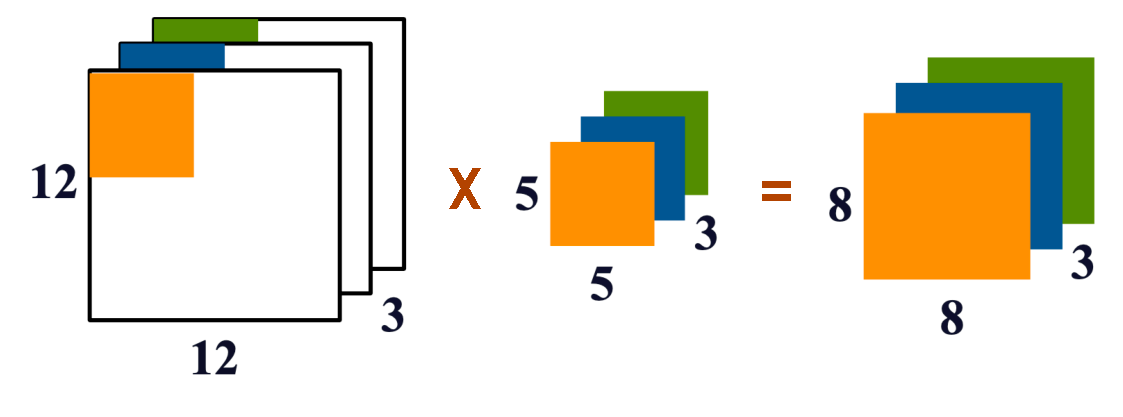
\includegraphics[height=2.5cm]{./figure/depthwisedemo.eps}
	\label{fig:dwdemo}}
\vspace{1em}
\subfloat[Pointwise convolution: four 3-channel $1 \times 1$ filters are used to convolve with one 3-channel $8 \times 8$ input and generate one 4-channel $8 \times 8$ output.]{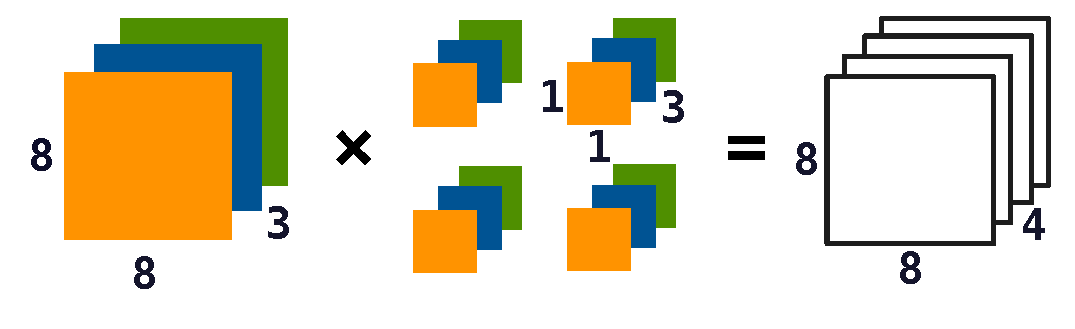
\includegraphics[height=2.5cm]{./figure/pointwisedemo.eps}
	\label{fig:pwdemo}}
\caption{Demonstration of depthwise and pointwise convolutions.}
  \label{fig:depsepconv}
\end{figure}

\subsection{Depthwise Separable Convolution}
Our work targets depthwise separable convolution (DSC) that is widely used by  CNN  models to reduce the number of multiplication
operations needed for doing convolution (a standard operation in CNN). The DSC splits a standard (e.g., multi-channeled) 2D
convolution kernel into two individual kernels: a depthwise convolution kernel and a pointwise convolution kernel. 

The depthwise
convolution kernel processes one input channel at a time, and stacks the outputs of all channels together to form an $n \times n \times c$
matrix, where $n \times n$ is the output of a depthwise convolution kernel and $c$ is the number of channels to be processed. Specifically,
it takes as input a feature map and applies a bank of 2D filters (e.g., an $N \times N$ kernel) on the width and height directions of
the input. We iteratively apply the depthwise convolution kernel to all channels. Fig. \ref{fig:dwdemo} shows an example of depthwise convolution, where three $5 \times 5$ 2D filters are used to convolve with the corresponding channel of a $12 \times 12 \times 3$ feature map and generate one $8 \times 8 \times 3$ output. 

The output of the depthwise convolution kernel is fed
into a pointwise convolution kernel which uses a $1 \times 1$ filter to iterates through every single point. This kernel has a depth of the
number of input channels (i.e., $c$). The DSC reduces the computation by reducing the number of input transformations needed when compared
to a standard depthwise convolution. Fig. \ref{fig:pwdemo} shows an example of pointwise convolution, where four $1 \times 1 \times 3$ filters are used to convolve with the $8 \times 8 \times 3$ feature map iteratively and each filter generate one channel of a $8 \times 8 \times 3$ output.


\subsection{Roadmap and Notations} We present our approach for optimizing the two convolutional kernels of DSC in
Sections \ref {sec:strategies} and \ref {sec:pwconv}. We start by introducing our methods for improving data locality of depthwise
convolution in Section \ref{sec:strategies} and then presenting our approach for using dynamic work distribution to accelerate
small-batch-sized pointwise convolution in Section \ref {sec:pwconv}.

\mypara{Notations.} Throughout the paper, we use $I$, $F$, and $O$ to represent the input, the filter, and the output respectively; we also
use $N$, $C$, $H$, and $W$ to denote the batch size, the channel, the height, and the width, respectively.

\section{Related Work}
Numerous efforts have been dedicated to optimizing convolution operations. As previously mentioned, GEMM-, FFT- and
Winograd-based convolutions are broadly adopted convolution algorithms.

GEMM-based convolution is the first attempt to optimize convolution. Chellapilla et al. \cite{Chellapilla2006High} developed an unrolling
convolution algorithm  called the im2col convolution algorithm. They lowered the convolutions into a matrix multiplication, which is
highly optimized on GPUs. Despite some duplicate input elements involved in the computation, the performance gain of this algorithm is impressive.

FFT- and Winograd-based convolutions can reduce computational complexity and improve convolution performance. Mathieu et al.
\cite{mathieu2013fast} proposed an FFT-based convolution to compute convolutions as pointwise products in the Fourier domain and reuse the
transformed input data, which significantly reduces the complexity of the convolution. However, FFT-based convolution is more suitable for large filters than
for small ones. Because padding the filters to the same size as the input data is necessary, and  the latter (e.g., $3 \times 3$ filters) needs
more memory than the former. Lavin et al. \cite{lavin2016fast} used Winograd's minimal filtering algorithm to
accelerate the convolution on GPU. This algorithm can reduce the arithmetic complexity of convolution by up to four times compared with
direct convolution. However, Winograd's algorithm is only suitable for small filters due to its numerical instability.
Zhen et al. \cite{Zhen2018Optimizing} extended Winograd's algorithm to support any filter size. However, the traditional and extended Winograd-based
algorithms need to transform the input and filter before performing matrix multiplication, and both require more operations than the FFT algorithm.

Transforming the input and filter before performing matrix multiplication incurs a large memory overhead, which can outweigh the
performance gains obtained through lowering the computational complexity. Therefore, recent studies have looked into minimizing the memory
overhead of the transformation phases. Cho et al. \cite{cho2017mec} reduced the memory overhead of GEMM-based convolutions using a compact
lowering scheme to reduce the redundancy in the lowered matrix and then performed multiple small matrix multiplications in parallel.
However, this algorithm still needs to transform the input and filter tensors into lowered matrixes to compute the convolution. Iandola et
al. \cite{Iandola2014Communication} reduced memory communication of 2D convolutions on GPU. They also prefetched the image regions to the
registers. While their method uses fewer threads, each thread operates on a larger number of data items. As a result, their method does not
reduce the number of global memory transactions. Unlike \cite{Iandola2014Communication}, our approach promotes register use and can
significantly reduce the number of memory accesses.



%In contrast, our convolution algorithm does not need to do any transformations and reduce memory operations through shuffle instruction.


%\section{Background and Motivation}
%\subsection{Convolution Operation in cuDNN}
%\subsection{CUDA shfl Instruction}
%\subsection{Motivation}

\section{Memory Transaction Optimization}
\label{sec:strategies}
In this section, we elaborate on our two optimization algorithms. The key idea is to reduce the  number of memory transactions which leads to the improvement in performance. Based on the observations shown in Figure \ref{fig:twostrategies}, we propose two reuse algorithms, column reuse and row reuse, which can significantly reduce the number of memory transactions.


\subsection{Column Reuse}
\begin{figure*}
	\begin{subfigure}{0.33\textwidth}
		\centering
		\captionsetup{width=0.9\textwidth}
		 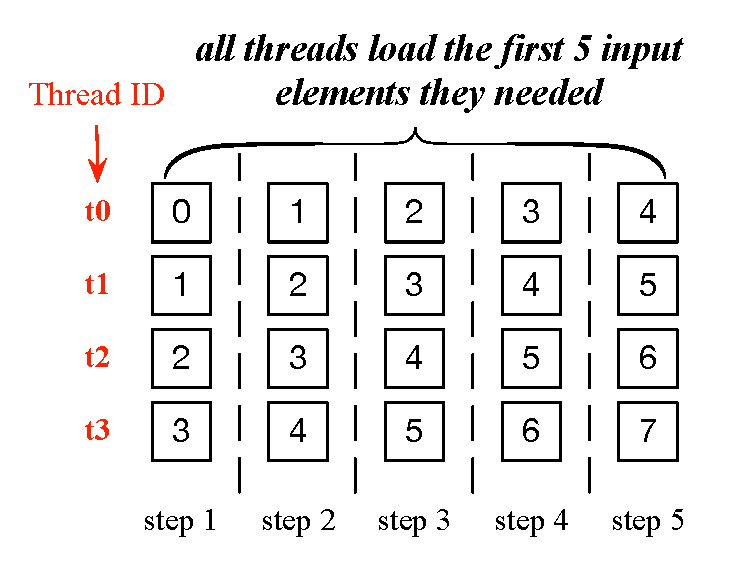
\includegraphics[width=0.98\textwidth,height=4.5cm]{./figure/directconv.eps}
		 \caption{Direct convolution: Each thread loads 5 input elements from global memory.}
		 \label{fig:directalgo}
	\end{subfigure}
	\begin{subfigure}{0.3\textwidth}
		\centering
		\captionsetup{width=0.9\textwidth}
		 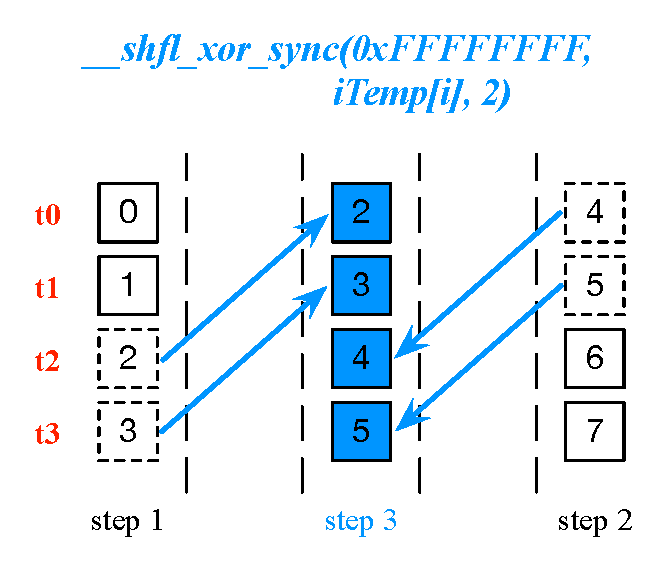
\includegraphics[width=\textwidth,height=4.5cm]{./figure/optalgo1.eps}
		 \caption{Optimized convolution: each thread retrieve its third element from the corresponding thread.}
		 \label{fig:optalgo1}
	\end{subfigure}
	\begin{subfigure}{0.3\textwidth}
		\centering
		\captionsetup{width=0.9\textwidth}

		 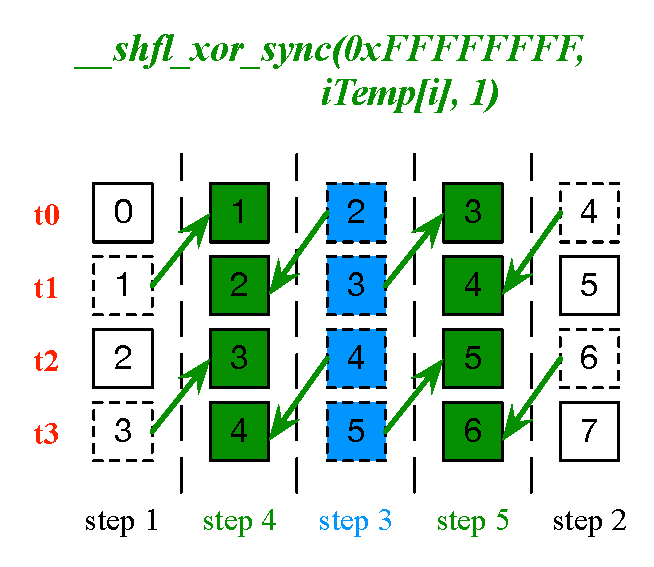
\includegraphics[width=0.96\textwidth,height=4.5cm]{./figure/optalgo2.eps}
		 \caption{Optimized convolution: each thread retrieve its second and fourth elements from corresponding threads.}
		 \label{fig:optalgo2}
	\end{subfigure}
  \caption{Illustration of direct and optimized convolution. We use a $5 \times 5$ filter  and each thread calculate convolution for one output element. Here we demonstrate how each thread processes first 5 corresponding input elements.}
   \label{fig:corealgo}
\end{figure*}

In this section, we demonstrate how to perform column reuse to eliminate duplicate columns. Using the convolution operation in Figure \ref{fig:twostrategies} as an example, we present the process of column reuse in Figure \ref{fig:corealgo}.%Each thread loads the first 5 corresponding input elements (each thread needs to load $F_H \times F_W \times F_C = 5 \times 5 \times 1 = 25$ input elements in total) to calculate the convolution of one output element.

\begin{figure}
	\centering
	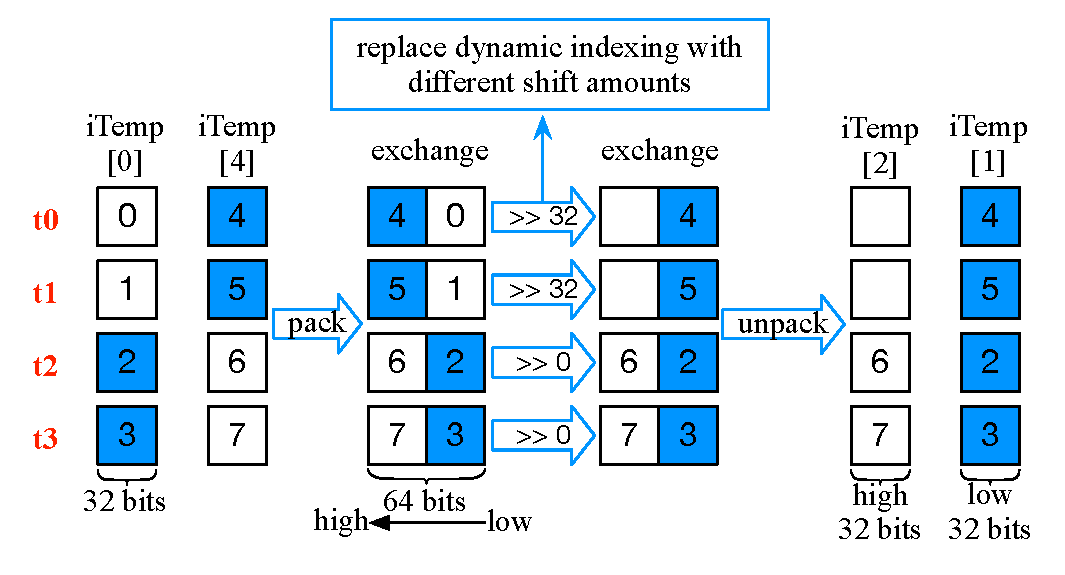
\includegraphics[width=\columnwidth,height=4.5cm]{./figure/exchange.eps}
\caption{Convert the dynamic indexing of array $iTemp$ into static indexing. Therefore, CUDA compiler can put $iTemp$ into registers instead of local memory.}
\label{fig:exchange}
\end{figure}


In step 1 of Figure \ref{fig:directalgo}, threads of the first warp load the first corresponding input elements from global memory. Because addresses of these elements are contiguous (0, 1, 2, 3), the warp can coalesce these accesses into one memory transaction. Therefore, 5 memory transactions are required for step 1-5 of Figure \ref{fig:directalgo}. Each pair of adjacent threads have four duplicate input elements, which corresponds to duplicate columns in Figure \ref{fig:twostrategies}. Next, we details how to eliminate this type of duplication.

As we can see from Figure \ref{fig:directalgo}, input elements 1, 2, 3 loaded in step 2 are already loaded by thread $t1$, $t2$, $t3$ in step 1. Therefore, we can retrieve input elements 1, 2, 3 from thread $t1$, $t2$, $t3$ instead of loading them from global memory (or L1 cache). This kind of duplication also occurs in step 3, 4, 5.

To eliminate redundant loads, we use CUDA shuffle instructions to exchange input elements between threads within the same warp. In step 1 and step 2 of Figure \ref{fig:optalgo1}, each thread loads its first and the fifth input elements from global memory. In step 3, each thread utilizes shuffle instruction to retrieve its third element from another thread. Threads $t0$ and $t1$ retrieve their third elements from threads $t2$ and $t3$ respectively, and also provide their fifth elements (shown as dashed square in step 2) for thread $t2$ and $t3$. In the meantime, threads $t2$ and $t3$ retrieve their third elements from threads $t0$ and $t1$ respectively, and also provide their first elements (shown as dashed square in step 1) for threads $t0$ and $t1$. This exchange process can be implemented using the instruction $shfl\_xor(iTemp[i],2)$ (the exact form of shuffle instructions can be found at \cite{CUDAtoolkit}), where $iTemp$ is the thread local array used to store five input elements and $i$ indexes which element to provide. For threads $t0$ and $t1$, both need to provide the fifth elements, therefore $i=4$. For threads $t2$ and $t3$, both need to provide the first elements, therefore $i=0$. Figure \ref{fig:optalgo2} has the similar procedure as Figure \ref{fig:optalgo1}, the difference is that each thread in Figure \ref{fig:optalgo2} retrieve its second and fourth elements from its neighboring threads.


However, the instruction $shfl\_xor(iTemp[i],2)$ significantly degrades the performance of convolution. Because $iTemp$ is an array with dynamic indexing, which means that CUDA compiler can not decide which element to provide at compile time. Therefore CUDA compiler will place array $iTemp$ in local memory which has the same access latency as global memory, instead of registers. This will significantly increase the memory access time and degrade the performance of convolution.

\begin{algorithm}
	$tid \gets threadIdx.x$\;
	$iTemp[0] \gets iData[iIndex]$\;
	$iTemp[4] \gets iData[iIndex+4]$\;
	$mov\ exchange, \{iTemp[0], iTemp[4]\}$\;
	$shift \gets ((tid+2)\&2)<<4$\;
	$exchange \gets exchange >> shift$\;
	$mov\ \{iTemp[1],iTemp[2]\}, exchange$\;
	$iTemp[2] \gets shfl\_xor(iTemp[1],2)$\;	
	
	\caption{Data exchange algorithm for retrieving the third element}
	\label{algo:basic}
\end{algorithm}

To convert dynamic indexing into static indexing, we design Algorithm \ref{algo:basic} for step 3 in Figure \ref{fig:optalgo1} and Algorithm \ref{algo:basic2} for step 4 and 5 in Figure \ref{fig:optalgo2}. Both algorithms use the same method but deal with different situations. Both algorithms can change dynamic indexing into static indexing and reduce the number of memory accesses. We use Algorithm \ref{algo:basic} as an example to illustrate how to eliminate dynamic indexing.

Figure \ref{fig:exchange} illustrates the process of Line 4-7 of Algorithm \ref{algo:basic}. Each thread loads the first and fifth corresponding input elements into thread local array $iTemp$ (Line 2-3). Then, pack both 32-bit elements into a 64-bit variable $exchange$ where $iTemp[4]$ is the high 32 bits and $iTemp[0]$ is the low 32 bits (Line 4). As threads $t0$ and $t1$ need to provide the their fifth elements which are high 32 bits of $exchange$, we right shift $exchange$ by 32 to put $iTemp[4]$ in low 32 bits. For threads $t2$ and $t3$, both need to provide their first elements which are already low 32 bits of $exchange$. therefore we right shift $exchange$ in threads $t2$ and $t3$ by 0. Shift amounts of each thread is calculated based on the thread id (Line 5). Afterwards, unpack $exchange$ into $iTemp[2]$ (high 32 bits) and $iTemp[1]$ (low 32 bits) (Line 7). And $iTemp[1]$ is the element that each thread needs to provide. Finally, using shuffle instruction to exchange elements between threads (Line 8).

Compared with the previous usage of shuffle instruction \cite{vasilache2014fast}, Algorithm \ref{algo:basic} successfully replace dynamic indexing $i$ in $shfl\_xor(iTemp[i],2)$ with static indexing $1$ in $shfl\_xor(iTemp[1],2)$.
Algorithm \ref{algo:basic} successfully eliminates dynamic indexing and therefore all thread local variables can be put in registers, which significantly improve the performance of convolution.

\begin{algorithm}
	$tid \gets threadIdx.x$\;
	$mov\ exchange, \{iTemp[0], iTemp[2]\}$\;
	$shift \gets ((tid+1)\&1)<<5$\;
	$exchange \gets exchange >> shift$\;
	$mov\ \{iTemp[0],iTemp[1]\}, exchange$\;
	$iTemp[1] \gets shfl\_xor(iTemp[0],1)$\;	
	\caption{Data exchange algorithm for retrieving the second element}
	\label{algo:basic2}
\end{algorithm}

Step 4 and step 5 in Figure \ref{fig:optalgo2} have similar procedure as step 3 in Figure \ref{fig:optalgo1}. Thus, we slightly modify Algorithm \ref{algo:basic} to obtain Algorithm \ref{algo:basic2}. The main distinction is that four threads are involved to exchange elements in Figure \ref{fig:optalgo1} while only two adjacent threads are involved in Figure \ref{fig:optalgo2}. Accordingly, we need to recalculate shift amounts for each thread (Line 3) and change arguments of the shuffle instruction (Line 6).

In summary, with Algorithm \ref{algo:basic} and \ref{algo:basic2}, we can reduce the number of memory transactions from 5 to 2 when loading 5 input elements and from 25 to 10 when loading 25 input elements. This reduction in the number of memory transactions brings a significant performance improvements for convolution.

\subsection{Row Reuse}
\begin{figure}
	\centering
	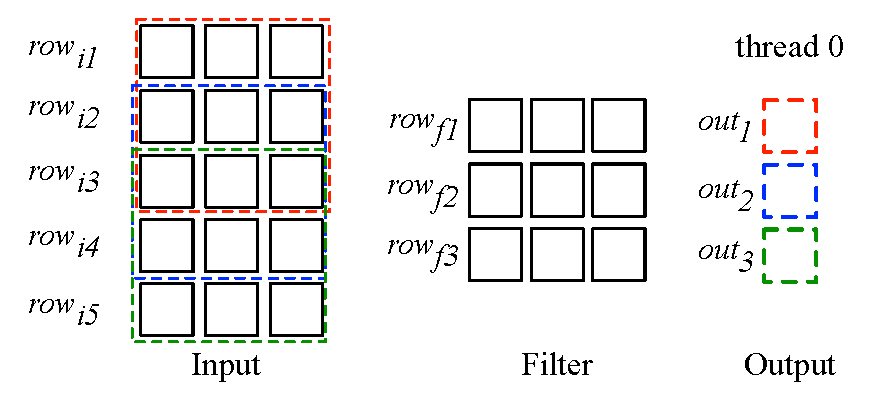
\includegraphics[width=\columnwidth,height=3.7cm]{./figure/rowreuse.eps}
\caption{A $3 \times 3$ filter is used to slide over the input image along height dimension and produce a column of output elements. One CUDA thread is used to calculate this column of output elements.}
\label{fig:rowreuse}
\end{figure}

When sliding the filter over the input image along height dimension, we can get a column of output elements, as shown in Figure \ref{fig:rowreuse}. In our design, we use one CUDA thread to calculate one column of output elements. Based on Figure \ref{fig:rowreuse}, we can perform convolution as follows:

\begin{gather*}
  out_1=row_{i1} \cdot row_{f1} + row_{i2} \cdot row_{f2} + row_{i3} \cdot row_{f3} \\
out_{2}=row_{i2} \cdot row_{f1} + row_{i3} \cdot row_{f2} + row_{i4} \cdot row_{f3} \\
	out_{3}=row_{i3} \cdot row_{f1} + row_{i4} \cdot row_{f2} + row_{i5} \cdot row_{f3}
\end{gather*}

From above equations, we can see that $row_{i2}$ and $row_{i4}$ are loaded twice, $row_{i3}$ is loaded three times. We need to load 9 rows in total. To eliminate row duplications, we redesign the way to perform convolution. After loading a row from input, we first determine how many output elements need this row. For example, $row_{i1}$ is needed by $out_1$, $row_{i2}$ is needed by $out_1$ and $out_2$. Then, we use this row to do inner product with corresponding rows of the filter to calculate output elements which need this row. Resigned formulations are shown as follows:
\begin{equation}\nonumber
\begin{aligned}
load\ row_{i1}:
&\ out_1=row_{i1} \cdot row_{f1} \\
load\ row_{i2}:
&\ out_1 = out_1+row_{i2} \cdot row_{f2}\\
&\ out_2=row_{i2} \cdot row_{f1}\\
load\ row_{i3}:
&\ out_1 = out_1+row_{i3} \cdot row_{f3}\\
&\ out_2 = out_2+row_{i3} \cdot row_{f2}\\
&\ out_{3}=row_{i3} \cdot row_{f1}\\
load\ row_{i4}:
&\ out_2=out_2+row_{i4} \cdot row_{f3} \\
&\ out_3=out_3+row_{i4} \cdot row_{f2}\\
load\ row_{i5}:
&\ out_3=out_3+row_{i5} \cdot row_{f3}
\end{aligned}	
\end{equation}



We can see from above equations that only 5 rows are loaded to calculate output elements. A more generalized description of the method is shown in Algorithm \ref{algo:rowreuse}, $row$ denotes the row loaded from the input, $index$ denotes the index of $row$, $filter$ denotes the vector of filter rows. Line 1-5 deals with the first $F_H-1$ rows ($row_{i1}$ and $row_{i2}$ in Figure \ref{algo:rowreuse}), these rows are needed by less than $F_H$ output elements. Line 6-11 deals with rows that are needed by exactly $F_H$ output elements ($row_{i3}$ in Figure \ref{algo:rowreuse}). Line 12-17 deals with last $F_H-1$ rows, these rows are needed by less than $F_H$ output elements ($row_{i4}$ and $row_{i5}$ in Figure \ref{algo:rowreuse}).

\begin{algorithm}
	\KwIn{$row$, $index$, $filter$, $Out$}
	\KwOut{$Out$}
	\If{$index \textless F_H-1$}{
		\For {$i \gets 0$ \KwTo $index+1$}{
			$Out[i] \gets Out[i]+row \cdot filter[index-i]$\;
		}
	}\ElseIf{$index \geq F_H-1$ \textbf{and} $index \textless I_H-F_H+1$}{
		\For {$i \gets 0$ \KwTo $F_H$}{
			$o_{index} \gets index-F_H+1+i$\;
			$Out[o_{index}] \gets Out[o_{index}]+row \cdot filter[F_H-1-i]$\;
		}
	}\Else{
		\For {$i \gets F_H-1$ \KwTo $0$}{
			$o_{index} \gets I_H-F_H+1$\;
			$Out[o_{index}] \gets Out[o_{index}]+row \cdot filter[F_H-i]$\;
		}
	}
	\caption{Row reuse}
	\label{algo:rowreuse}
\end{algorithm}

In summary, Algorithm \ref{algo:rowreuse} eliminates row duplications when sliding a filter over input along height dimension. The algorithm loads each row of input exactly once and thus greatly reduces the number of memory transactions.

\section{Memory Efficient Convolutions}
\begin{figure}
	\centering
	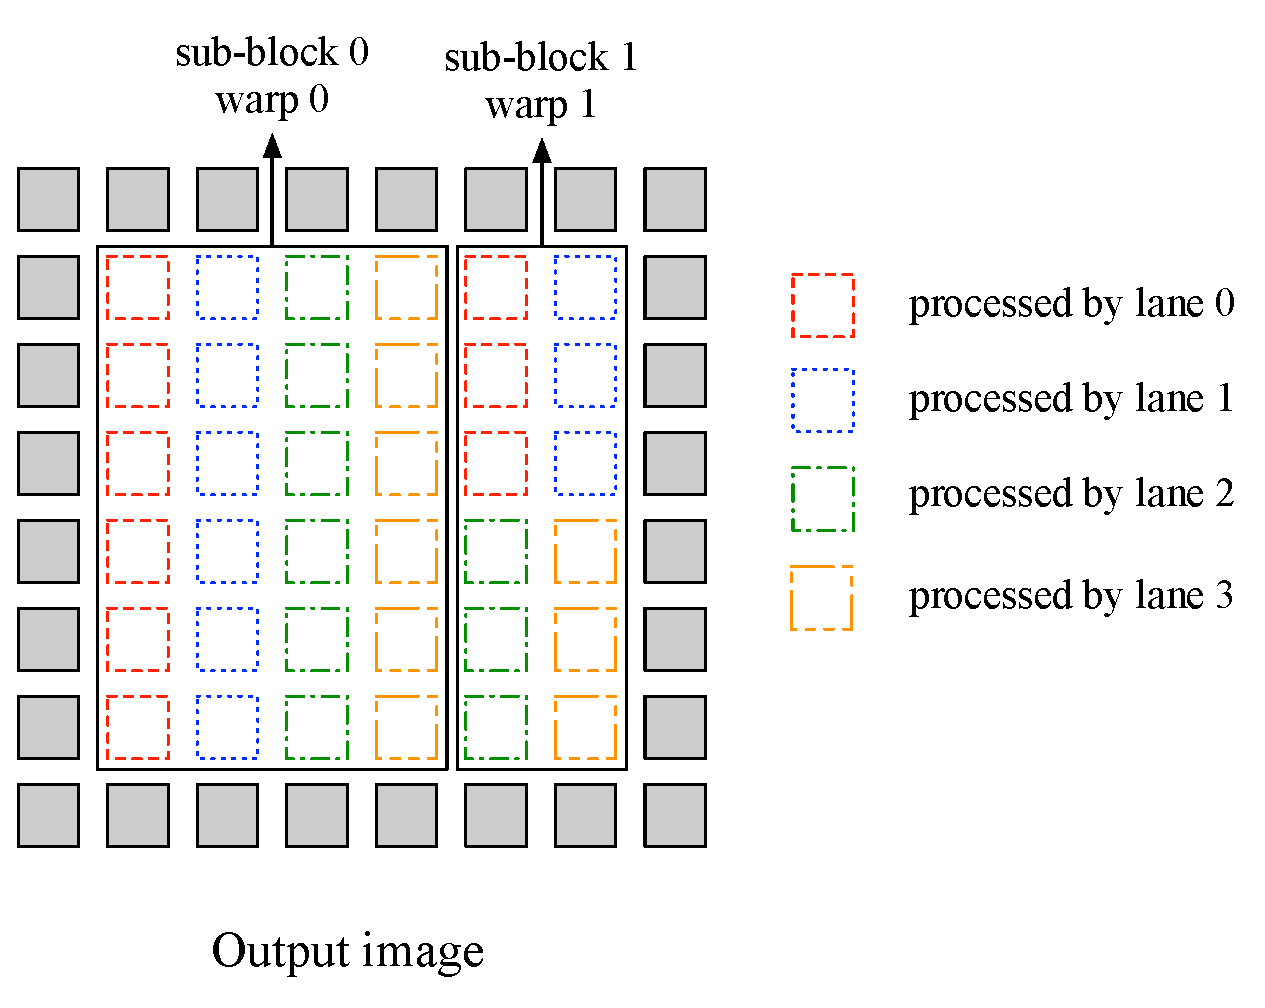
\includegraphics[width=0.9\columnwidth,height=5.5cm]{./figure/overalldesign.eps}
\caption{The output is produced by sliding a $3 \times 3$ filter over an $8 \times 8$ input with one pad. Edge elements and inner elements are processed by different CUDA thread blocks. We assume that warp size is 4 and thus $laneid=threadid\%4$.}
\label{fig:overalldesign}
\end{figure}


In this section, we demonstrate how to employ our two reuse algorithms on 2D and 3D convolutions. The main difference between implementations of 2D and 3D convolutions is how to load filters. For 2D convolution, we focus on the scenario where a filter is used to slide over a large image. Therefore, we can load the entire filter into shared memory and one CUDA thread block only needs to load the filter once. For 3D convolution, we focus on the scenario where many filters are used to slide over a batch of images. This is often the first layer of CNNs. The entire filters normally can not fit into the shared memory, thus we need to load filters multiple times.

To make this easily understood, we use 2D convolution as an example for illustration. In our implementation, we first divide the output into sub-blocks and each sub-block contains exactly 32 (warp size) columns except for the last sub-block which may contain less columns. Each CUDA thread block processes one or more sub-blocks and each warp process one sub-block. Threads within the same warp process adjacent columns of one sub-block.
\begin{algorithm}
	\KwIn{$I$, $F$, $O$, $subBlockHeight$}
	\KwOut{$O$}
	load filter into shared memory\;
	$\_\_syncthreads()$\;
	\If{$blockIdx.x \textless gridDim.x-1$}{
		Calculate the index of the first input element this thread needs, denoted as $baseIndex$\;
		\For{$i \gets 0$ \KwTo $I_C$}{
			$inputIndex \gets baseIndex+i*I_H*I_W$\;
			\For{$j \gets 0$ \KwTo $subBlockHeight$}{
				Use Algorithm \ref{algo:basic} and Algorithm \ref{algo:basic2} to load input elements the thread needs, the loaded elements are denoted as $row$\;
				
				Use Algorithm \ref{algo:rowreuse} to calculate output elements and store results into thread local register array $sum$\;
			}
		}
		Write array $sum$ into global memory\;
	}
	\Else{
		Process the remaining inner elements of $O$\;
		Process the edge elements of $O$\;
	}
	\caption{Overall design}
	\label{algo:overalldesign}
\end{algorithm}

Figure \ref{fig:overalldesign} is an illustration of how to map CUDA threads onto output elements. Since 2D convolution normally produces an output image of the same size as the input image, therefore we need to pad the input image. But we do not actually allocate memory on GPU, instead we use different methods to calculate edge and inner elements of the output image. In Figure \ref{fig:overalldesign}, edge elements and inner elements are denoted as shaded squares and dashed squares respectively.

We demonstrate how to deal with inner elements in this paper and we calculate edge elements with a similar method as inner elements. In Figure \ref{fig:overalldesign}, we assume that each warp contains 4 threads. We can see that the inner elements are divided into two sub-blocks. Sub-block 0 contains 4 columns which is exactly the warp size. Sub-block 1 contains only 2 columns, to make full use of threads within a warp, we divide the last two columns evenly among 4 threads. A generalized overall design is shown in Algorithm \ref{algo:overalldesign}.

In Algorithm \ref{algo:overalldesign}, we first load the filter into shared memory (Line 1-2). Then we process sub-blocks with exact 32 columns in Line 3-13 and the last sub-block in Line 14-17. Each thread calculates one column of output elements as follows: First, each thread calculates the address of the first input element it needs (Line 4-6); Second, each thread uses Algorithm \ref{algo:basic} and Algorithm \ref{algo:basic2} to fulfill the vector $row$ which contains a row of the sub-block (Line 8); Third, each thread passes the vector $row$ to Algorithm \ref{algo:rowreuse} to calculate multiple output elements and store results in register array $sum$ (Line 9); Last, each thread writes the result array $sum$ into global memory (Line 12).

\section{Evalution}
We evaluate our implementations of convolution on two platforms: (a) NVIDIA Tesla K40m facilitates 2880 FP32 cores with 64KB L1 cache and shared memory. The host machine has a 2.40GHz Intel Xeon E5-2620 CPU with 128GB memory and Linux kernel v4.19.85. (b) NVIDIA RTX 2080 Ti facilitates 4350 FP32 cores and 4350 INT32 cores with 96KB L1 cache and shared memory. The host machine has a 2.30GHz Intel Xeon E5-2697 CPU with 252GB memory and Linux kernel v4.15.0. Both platforms are shipped with the CUDA Toolkit v10.1. We use following state-of-the-art convolution libraries as a comparison on both platforms:
\begin{itemize}
  \item cuDNN, version 7.6. cuDNN is the state-of-art convolution implementation. It supports both 2D and 3D convolutions on GPU. Moreover, cuDNN implements GEMM-based, FFT-based and Winograd-based convolutions.
  \item GEMM-im2col and GEMM-im2row (im2col and im2row for short). Both are GEMM-based convolutions and support 2D and 3D convolutions. We extract the implementations of im2col and im2row from Caffe \cite{jia2014caffe} and MatConvNet \cite{vedaldi15matconvnet} respectively.
  \item ArrayFire \cite{Yalamanchili2015}, version 3.6.4. ArrayFire is a popular image and signal processing library. It implements 2D convolution on GPU and can be easily invoked through an api. The semantics of 3D convolution of ArrayFire is not compatible with 3D convolutions in CNNs. Therefore we use ArrayFire only for 2D convolution. ArrayFire uses Just In Time (JIT) compiling for standard arithmetic operations, which means that the first run of an ArrayFire application will take a much longer time than the second run. Thus, we run ArrayFire twice in each test and take the second runtime.
  \item NVIDIA Performance Primitives (NPP), version 10.1. NPP is an image and signal processing library. We do not find functions for performing 3D convolution like cuDNN. Therefore we use NPP only for 2D convolution.

\end{itemize}

After years of updating, cuDNN has integrated seven widely used convolution algorithms. Therefore, cuDNN provides an option that uses heuristics to find the most suitable algorithm for a convolution. We set the option to $PREFER\_FASTEST$ (the exact option can be found at \cite{CUDAtoolkit}) meaning that we want to use the fastest algorithm without regarding the memory capacity. However, the algorithm selected by the heuristic is not always the fastest. Therefore, we use two types of runtime for cuDNN. One is the real fastest runtime among seven algorithms and the other is heuristically fastest. For 2D convolution, we use the real fastest runtime since two types of runtime are the same.

%Our implementations of convolution use only a small part of shared memory and mainly relay on GPU L1 cache. Therefore we employ $cudaDeviceSetCacheConfig$ function to set GPU cache policy with arguments $cudaFuncCachePreferL1$ for our convolutions.
All experiments use 32-bit float data type and use the average runtime of 10 iterations. All data are 4-dimension tensors $(N,C,H,W)$. For now, we implement a 2D convolution and 3D convolutions with one and three input channels for filters of size $3 \times 3$ and $5 \times 5$, since small filters are commonly used in applications. We first present results for 2D convolution and then 3D convolution.

\subsection{2D Convolution}
\begin{figure*}
\begin{subfigure}{\columnwidth}
		\centering
		 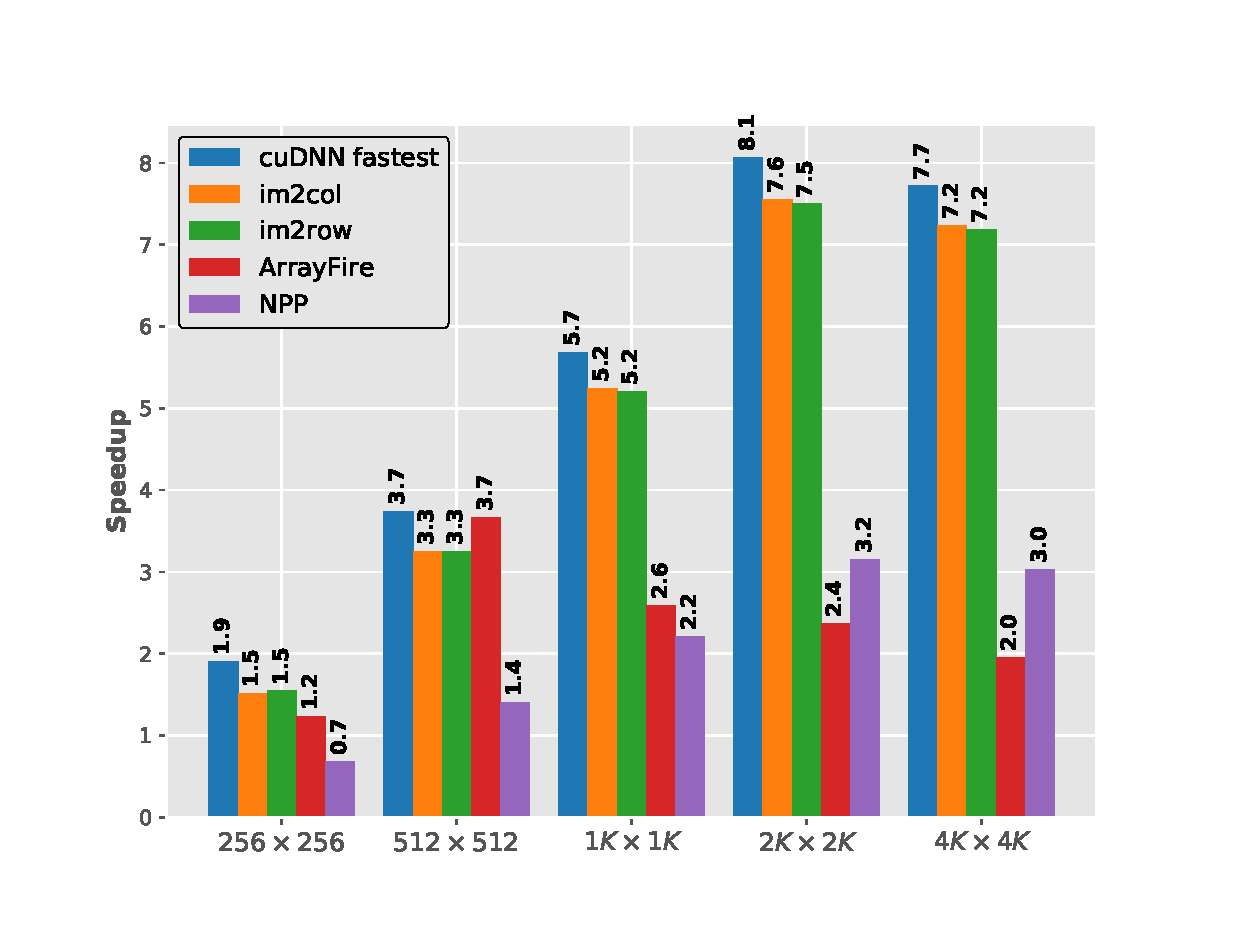
\includegraphics[width=\columnwidth,height=6cm]{./figure/2d_norm_f3.eps}
		 \caption{Speedups for the filter of size $3 \times 3$ on Tesla K40m.}
		 \label{fig:2druntimef3c1}
	\end{subfigure}
	\begin{subfigure}{\columnwidth}
		\centering
		 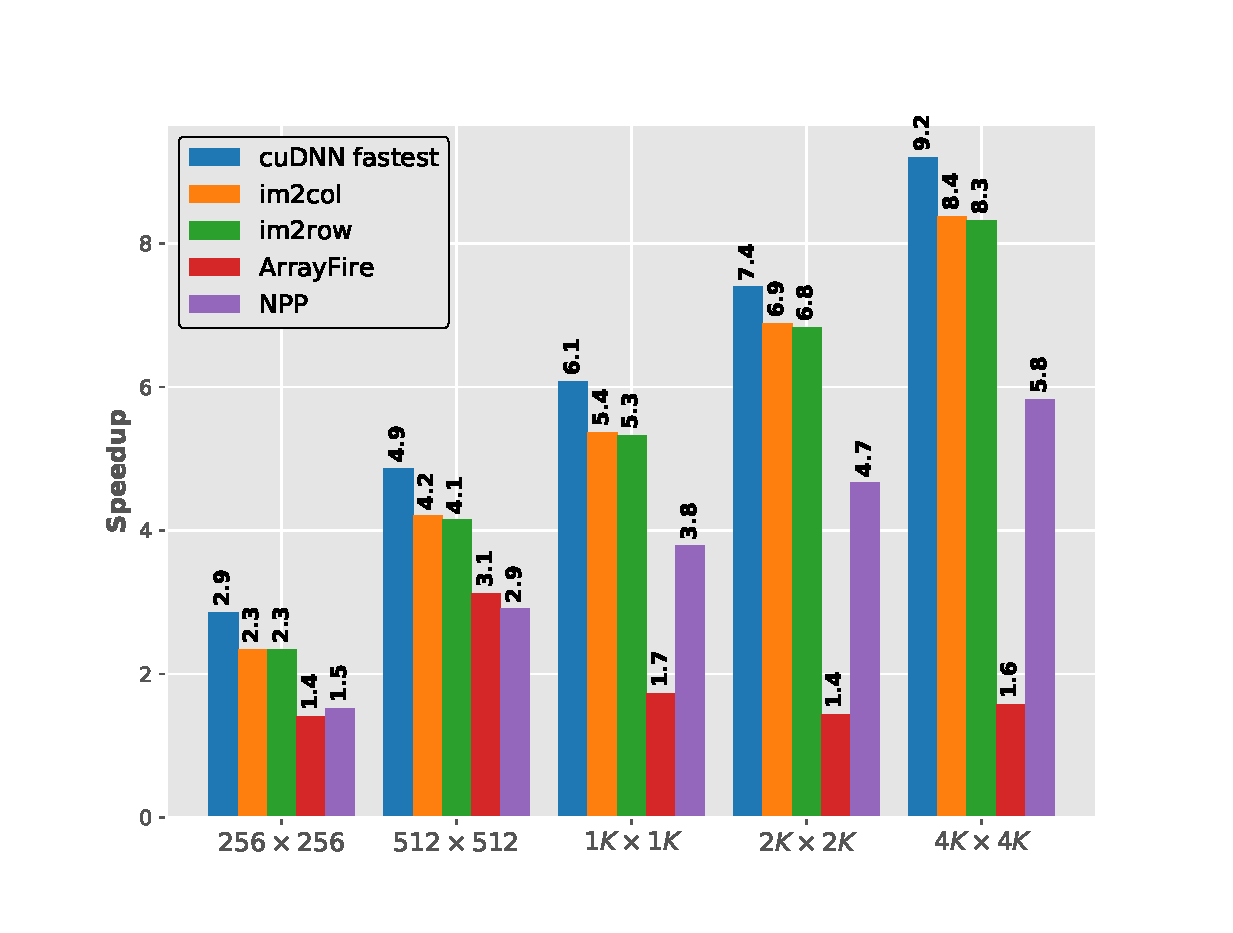
\includegraphics[width=\columnwidth,height=6cm]{./figure/2d_norm_f5.eps}
		 \caption{Speedups for the filter of size $5 \times 5$ on Tesla K40m.}
		 \label{fig:2druntimef5c1}
	\end{subfigure}
	
	\begin{subfigure}{\columnwidth}
		\centering
		 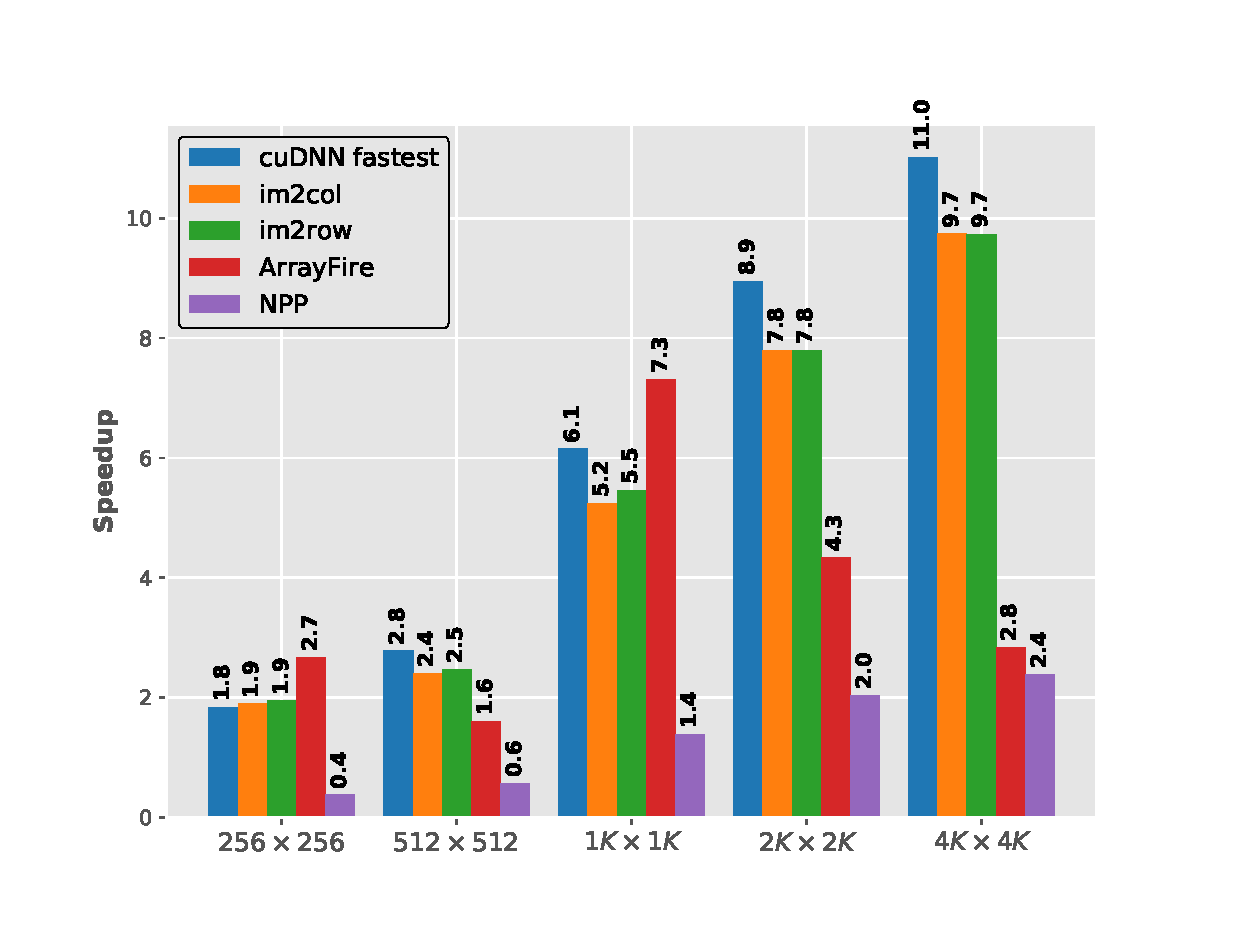
\includegraphics[width=\columnwidth,height=6cm]{./figure/2d_norm_f3_rtx2080.eps}
		 \caption{Speedups for the filter of size $3 \times 3$ on RTX 2080 Ti.}
		 \label{fig:2druntimef3c12080}
	\end{subfigure}
	\begin{subfigure}{\columnwidth}
		\centering
		 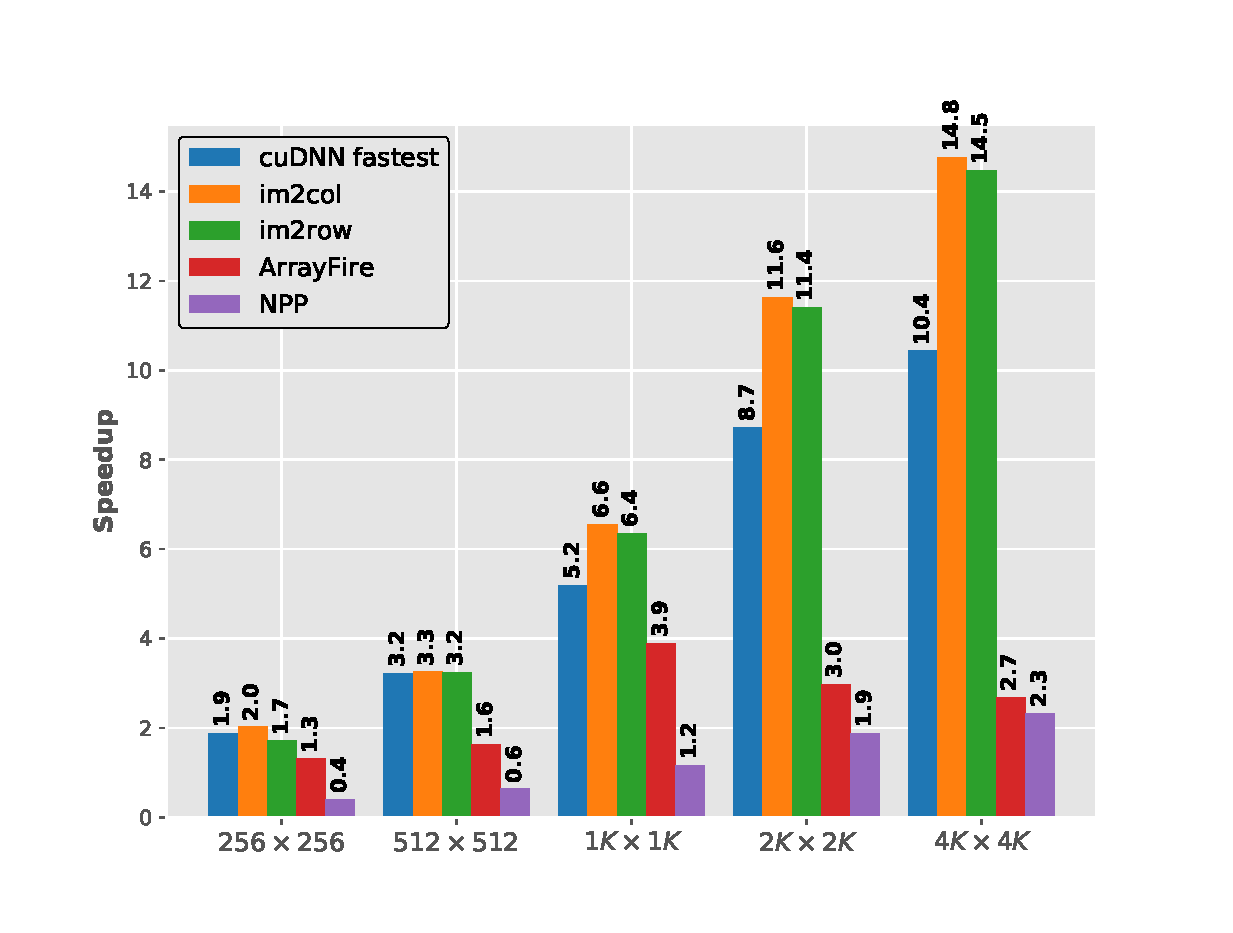
\includegraphics[width=\columnwidth,height=6cm]{./figure/2d_norm_f5_rtx2080.eps}
		 \caption{Speedups for the filter of size $5 \times 5$ on RTX 2080 Ti.}
		 \label{fig:2druntimef5c12080}
	\end{subfigure}
	
	\caption{Speedups of our implementation over the other five 2D convolution implementations on two platforms.}
   \label{fig:2druntime}
\end{figure*}

\begin{table*}[]
\caption{Summation of memory transactions on each type of memory, including global memory, texture memory and shared memory. Data is collected on Tesla K40m.}
\label{tab:2dmemtrans}
\begin{tabular}{c|ccccc|ccccc}
\hline
\multicolumn{1}{l|}{}                                  & \multicolumn{5}{c|}{Filter size $3 \times 3$}                                                & \multicolumn{5}{c}{Filter size $5 \times 5$}                                                \\ \hline
                                                       & $256 * 256$      & $512 * 512$      & $1K * 1K$        & $2K * 2K$        & $4K * 4K$        & $256 * 256$      & $512 * 512$      & $1K * 1K$        & $2K * 2K$        & $4K * 4K$        \\ \hline
cuDNN                                                  & 6.0E+05          & 2.4E+06          & 9.7E+06          & 3.9E+07          & 1.5E+08          & 1.4E+06          & 5.6E+06          & 2.2E+07          & 8.9E+07          & 3.6E+08          \\
 im2col & 1.1E+05          & 4.4E+05          & 4.4E+05          & 7.0E+06          & 2.8E+07          & 2.3E+05          & 9.3E+05          & 3.7E+06          & 1.5E+07          & 6.0E+07          \\
im2row & 1.1E+05          & 4.4E+05          & 4.4E+05          & 7.0E+06          & 2.8E+07          & 2.3E+05          & 9.3E+05          & 3.7E+06          & 1.5E+07          & 6.0E+07          \\
ArrayFire                                              & 4.9E+04          & 2.0E+05          & 7.9E+05          & 3.2E+06          & 1.3E+07          & 1.1E+05          & 4.2E+05          & 1.7E+06          & 6.8E+06          & 2.7E+07          \\
NPP                                                    & 6.0E+04          & 2.4E+05          & 9.6E+05          & 3.8E+06          & 1.5E+07          & 1.3E+05          & 5.2E+05          & 2.1E+06          & 8.3E+06          & 3.3E+07          \\
Ours                                                   & \textbf{7.5E+03} & \textbf{2.7E+04} & \textbf{1.1E+05} & \textbf{4.2E+05} & \textbf{1.6E+06} & \textbf{1.0E+04} & \textbf{3.3E+04} & \textbf{1.3E+05} & \textbf{4.9E+05} & \textbf{1.9E+06} \\ \hline
\end{tabular}
\end{table*}

In this section, we report the performance of 2D convolution obtained from six implementations, including cuDNN, im2col, im2row, ArrayFire, NPP and our implementation. We evaluate these six implementations with image size ($I_H \times I_W$) ranging from $256 \times 256$ to $4K \times 4K$, $I_N=F_N=1$ and $I_C=F_C=1$. We first present speedups of our implementation over the other five implementations in Figure \ref{fig:2druntime}. Then we show the effectiveness of our implementation on reducing the number of memory transactions in Table \ref{tab:2dmemtrans}.

It is apparent from Figure \ref{fig:2druntime} that cuDNN, im2col and im2row are not suitable for 2D convolution while ArrayFire, NPP and our implementation are well optimized for 2D convolution. Our implementation exhibits superior performance over cuDNN, im2col and im2row on two platforms with an average of 5.9$\times$, 5.9$\times$ and 5.8$\times$ speedups respectively.

Figure \ref{fig:2druntimef3c1} and \ref{fig:2druntimef5c1} show speedups on Tesla K40m,  we can see that our implementation achieves the best results in nine cases out of ten. Our implementation is only slower than NPP when performing $3 \times 3$ convolution on a $256 \times 256$ image. The average speedups of our implementation over ArrayFire and NPP on Tesla K40m are 2.1$\times$ and 2.9$\times$ respectively. Figure \ref{fig:2druntimef3c12080} and \ref{fig:2druntimef5c12080} show speedups on RTX 2080 Ti, our implementation achieves the best results in six cases out of ten. We can see that NPP achieves the best results on small image sizes while our implementation achieves the best results on large image sizes. The average speedups of our implementation over ArrayFire and NPP on RTX 2080 Ti are 3.1$\times$ and 1.3$\times$ respectively.

Our implementation of 2D convolution is derived from direct convolution. We employ only two optimization algorithms, column reuse (Algorithm \ref{algo:basic}, Algorithm \ref{algo:basic2}) and row reuse (Algorithm \ref{algo:rowreuse}) on direct convolution, therefore performance gains are mainly attributed to the reduction on the number of memory transactions. We use \emph{nvprof} provided by CUDA Toolkit to collect the number of memory transactions for different type of memories. GPU global memory is used to store input data in im2col, im2row, ArrayFire and our implementation. NPP and cuDNN use texture memory to store input data. Shared memory is normally used to store filter data. Therefore we sum up the number of read transactions of these three memory types and report the results in Table \ref{tab:2dmemtrans}. To save space, we only show the result of memory transactions collected on Tesla K40m, the result on RTX 2080 Ti exhibits the similar trend.

From Table \ref{tab:2dmemtrans} we can see that our optimization algorithms significantly reduce the number of memory transactions. Compared with ArrayFire and NPP which are well optimized for 2D convolution, our implementation can averagely reduce memory transactions by a factor of 10.2 and 12.3 respectively.


% Please add the following required packages to your document preamble:
% \usepackage{multirow}


%\begin{table*}[]
%\caption{2d speedup}
%\label{tab:2dspeedup}
%\begin{tabular}{c|ccccc|ccccc}
%\hline
%\multicolumn{1}{c}{}&\multicolumn{5}{c}{$F_H*F_W= 3*3$} &\multicolumn{5}{c}{$F_H*F_W= 5*5$}\\
%\hline
%           & 256*256&512*512&1K*1K&2K*2K&4K*4K&256*256&512*512&1K*1K&2K*2K&4K*4K\\
%\hline
%cuDNN      & 1.91 & 3.74 & 5.69 & 8.07 & 7.72     & 2.86 & 4.86 & 6.08 & 7.40 & 9.20  \\
%im2col     & 1.52 & 3.25 & 5.25 & 7.56 & 7.24     & 2.34 & 4.20 & 5.37 & 6.88 & 8.38  \\
%im2row     & 1.55 & 3.25 & 5.20 & 7.50 & 7.19     & 2.34 & 4.15 & 5.32 & 6.83 & 8.32  \\
%ArrayFire  & 1.23 & 3.67 & 2.59 & 2.37 & 1.95     & 1.40 & 3.12 & 1.73 & 1.43 & 1.57  \\
%NPP        & 0.68 & 1.40 & 2.21 & 3.15 & 3.03     & 1.52 & 2.91 & 3.79 & 4.66 & 5.82 \\
%\hline
%\end{tabular}
%\end{table*}
In summary, our optimization algorithms can significantly reduce the number of memory transactions and improve the performance of 2D convolution. Compared with state-of-the-art image processing libraries, ArrayFire and NPP, our implementation achieves average speedups of 2.1$\times$ and 2.9$\times$ on Tesla K40m, 1.3$\times$ and 3.1$\times$ on RTX 2080 Ti.

\subsection{3D Convolution}

\begin{table}[]
\caption{Configurations of 3D convolution}
\label{tab:3dconvconfigs}
\begin{tabular}{c|ccccc}
\hline
& $I_N$ & $I_C=F_C$ & $I_H*I_W$ & $F_N$ & $F_H*F_W$ \\
\hline
CONV1 & 128  & 1,3       & 28*28     & 128  & 3*3       \\
CONV2 & 128  & 1,3       & 56*56     & 64   & 3*3       \\
CONV3 & 128  & 1,3       & 12*12     & 64   & 5*5       \\
CONV4 & 128  & 1,3       & 14*14     & 16   & 5*5       \\
CONV5 & 128  & 1,3       & 24*24    & 256  & 5*5       \\
CONV6 & 128  & 1,3       & 24*24     & 64   & 5*5       \\
CONV7 & 128  & 1,3       & 28*28     & 16   & 5*5       \\
CONV8 & 128  & 1,3       & 28*28     & 512   & 3*3       \\
CONV9 & 128  & 1,3       & 56*56     & 256  & 3*3       \\
CONV10 & 128  & 1,3       & 112*112     & 128   & 3*3       \\
CONV11 & 128  & 1,3       & 224*224     & 64   & 3*3      \\
\hline
\end{tabular}
\end{table}

\begin{figure*}
	
		%\centering
		 %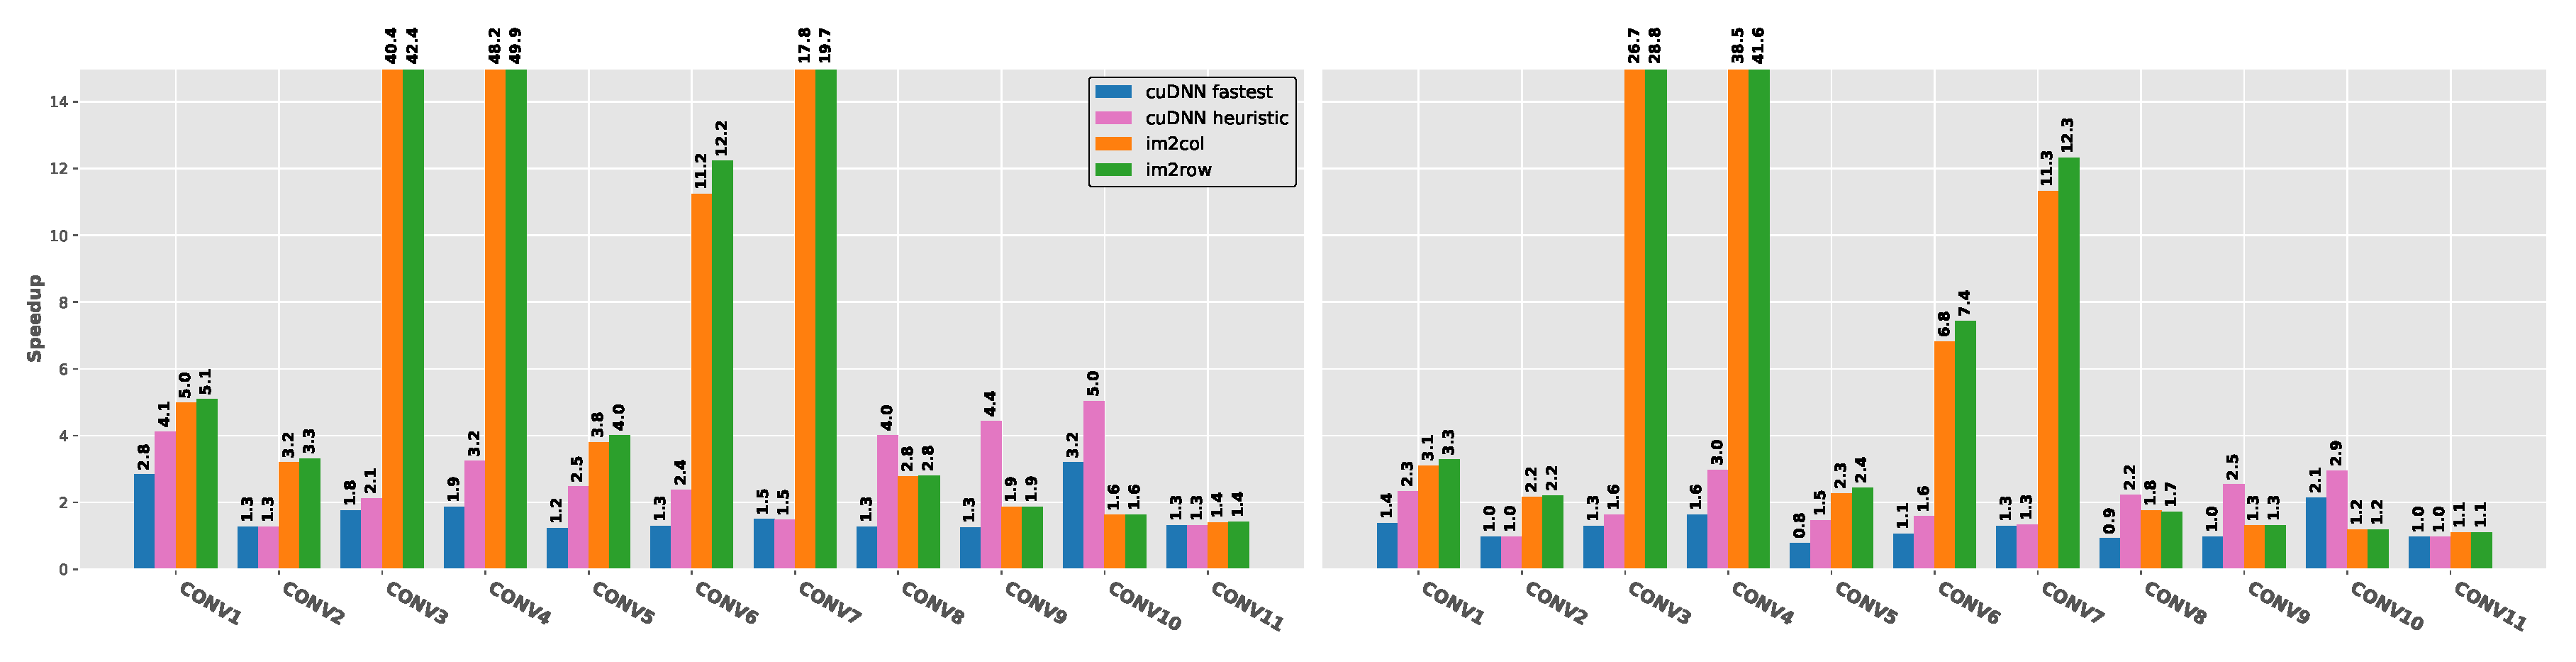
\includegraphics[width=18cm,height=5cm]{./figure/3d_norm_c1.eps}
		 %\caption{Normalized runtime of five implementations for 3D convolution. Left and right parts of the figure is for 3D convolutions with one and three input channels.}
		 %\label{fig:3druntime}
		
	\begin{subfigure}{18cm}
		\centering
		 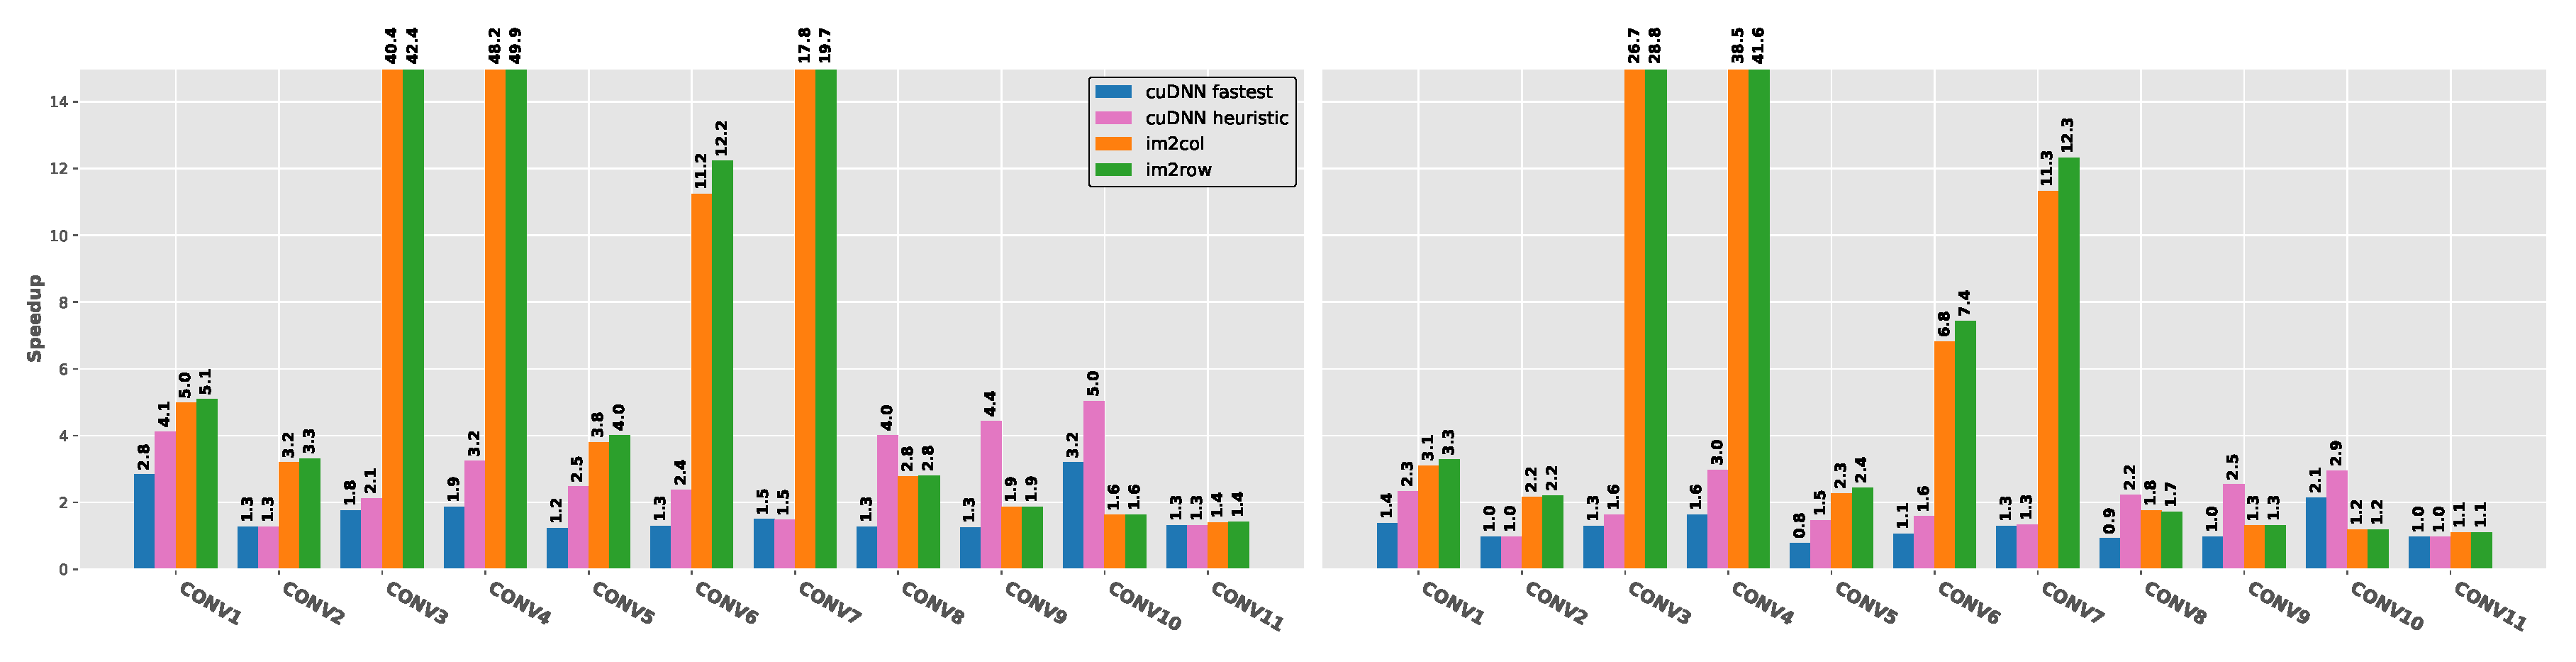
\includegraphics[width=18cm,height=5.7cm]{./figure/3d_norm_c1.eps}
		 \caption{Speedups on Tesla K40m, left is for one channel and right is for three channels.}
		 \label{fig:3druntimeK40}
	\end{subfigure}
	
	\begin{subfigure}{18cm}
		\centering
		 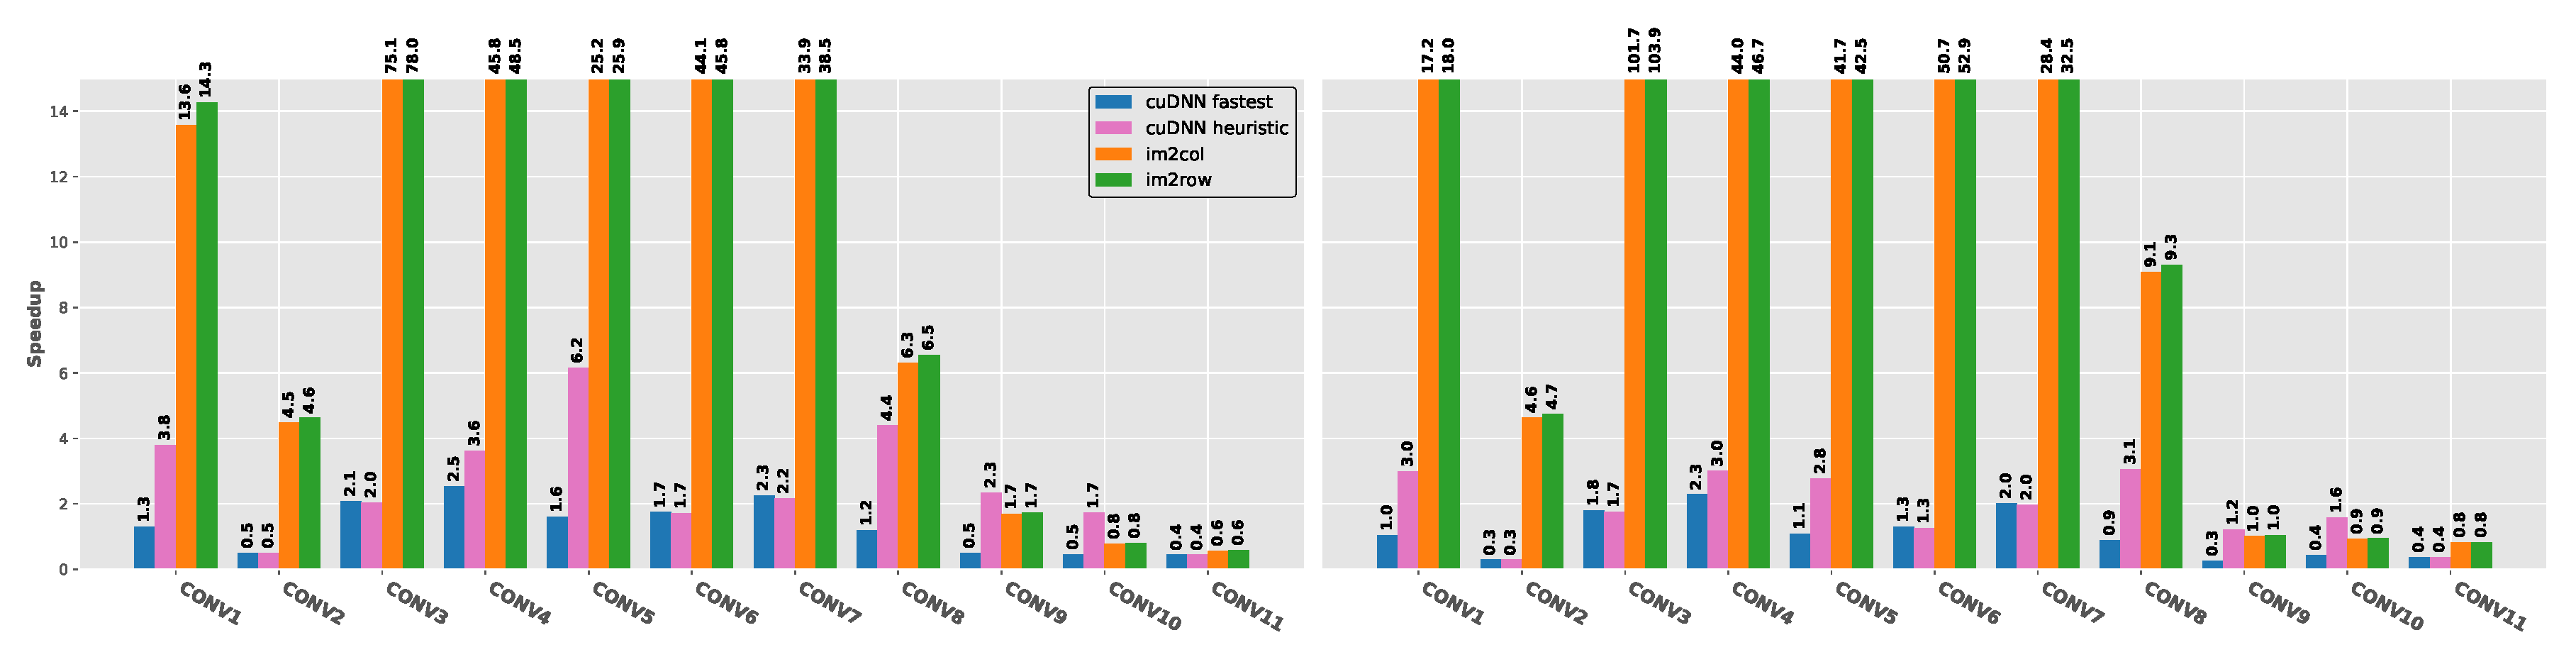
\includegraphics[width=18cm,height=5.7cm]{./figure/3d_norm_c1_rtx2080.eps}
		 \caption{Speedups on RTX 2080 Ti, left is for one channel and right is for three channels.}
		 \label{fig:3druntime2080}
	\end{subfigure}
	
	\caption{Speedups of our implementation over the other four implementations for 3D convolution with one and three input channels.}
	\label{fig:3druntime}
\end{figure*}
%\begin{figure*}
%	\begin{subfigure}{\columnwidth}
%		\centering
%		 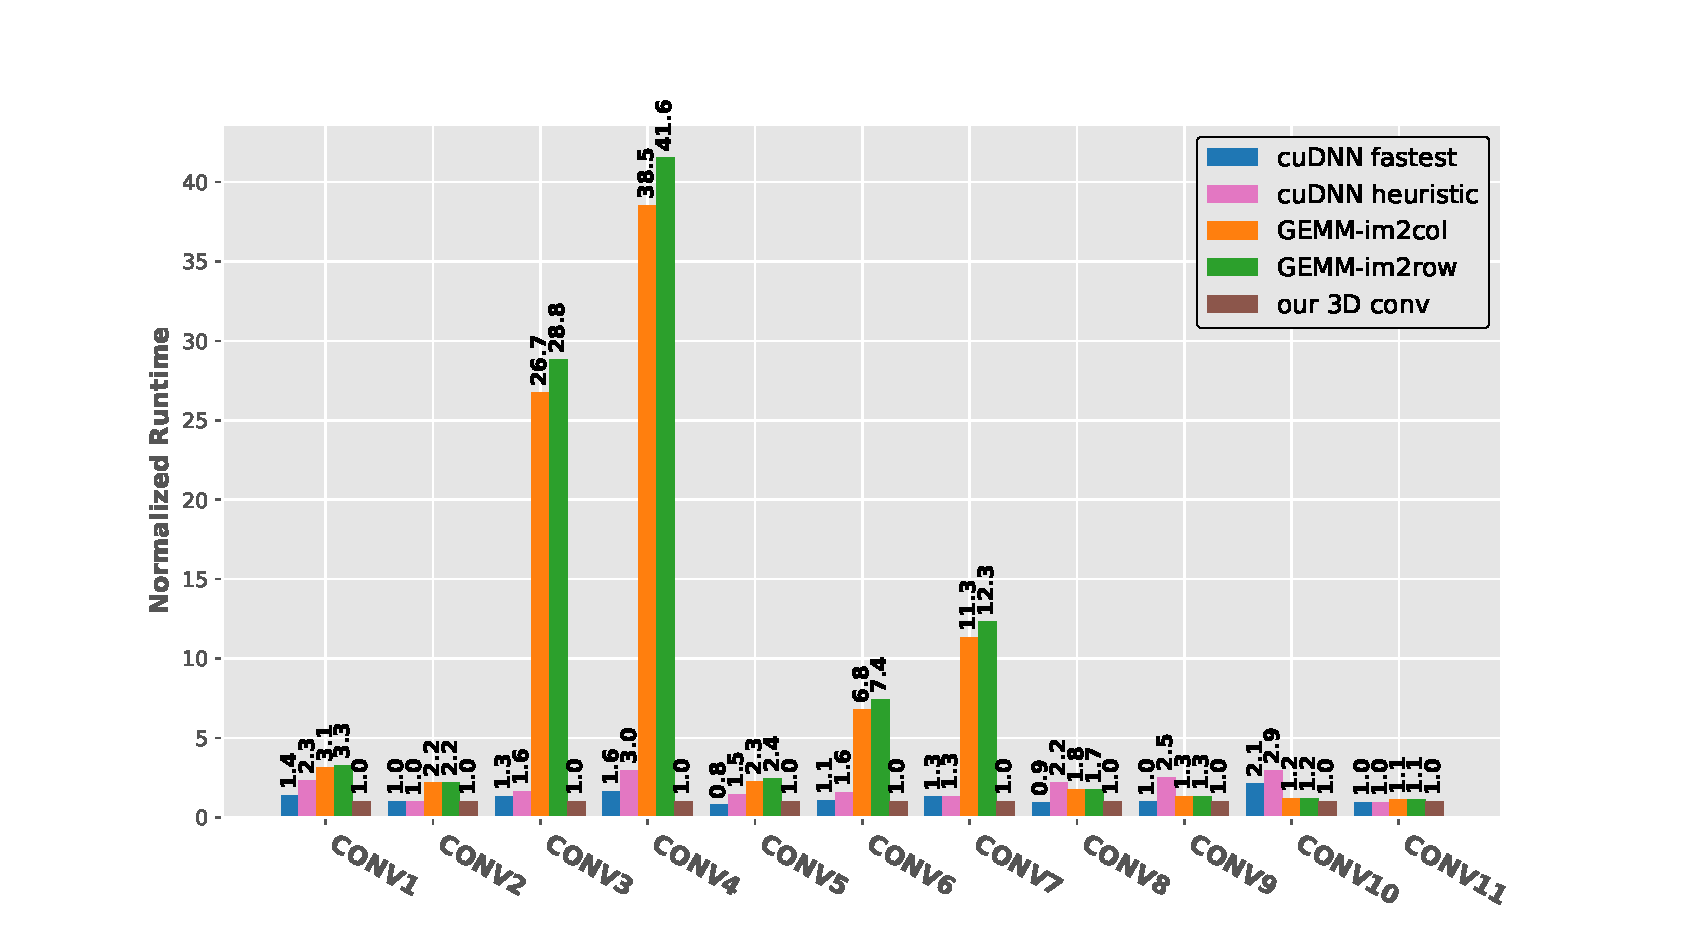
\includegraphics[width=\columnwidth,height=5cm]{./figure/3d_norm_c3.eps}
%		 \caption{Normalized runtime for convolutions with one input channel.}
%		 \label{fig:3druntimec1}
%	\end{subfigure}
%	\begin{subfigure}{\columnwidth}
%		\centering
%		 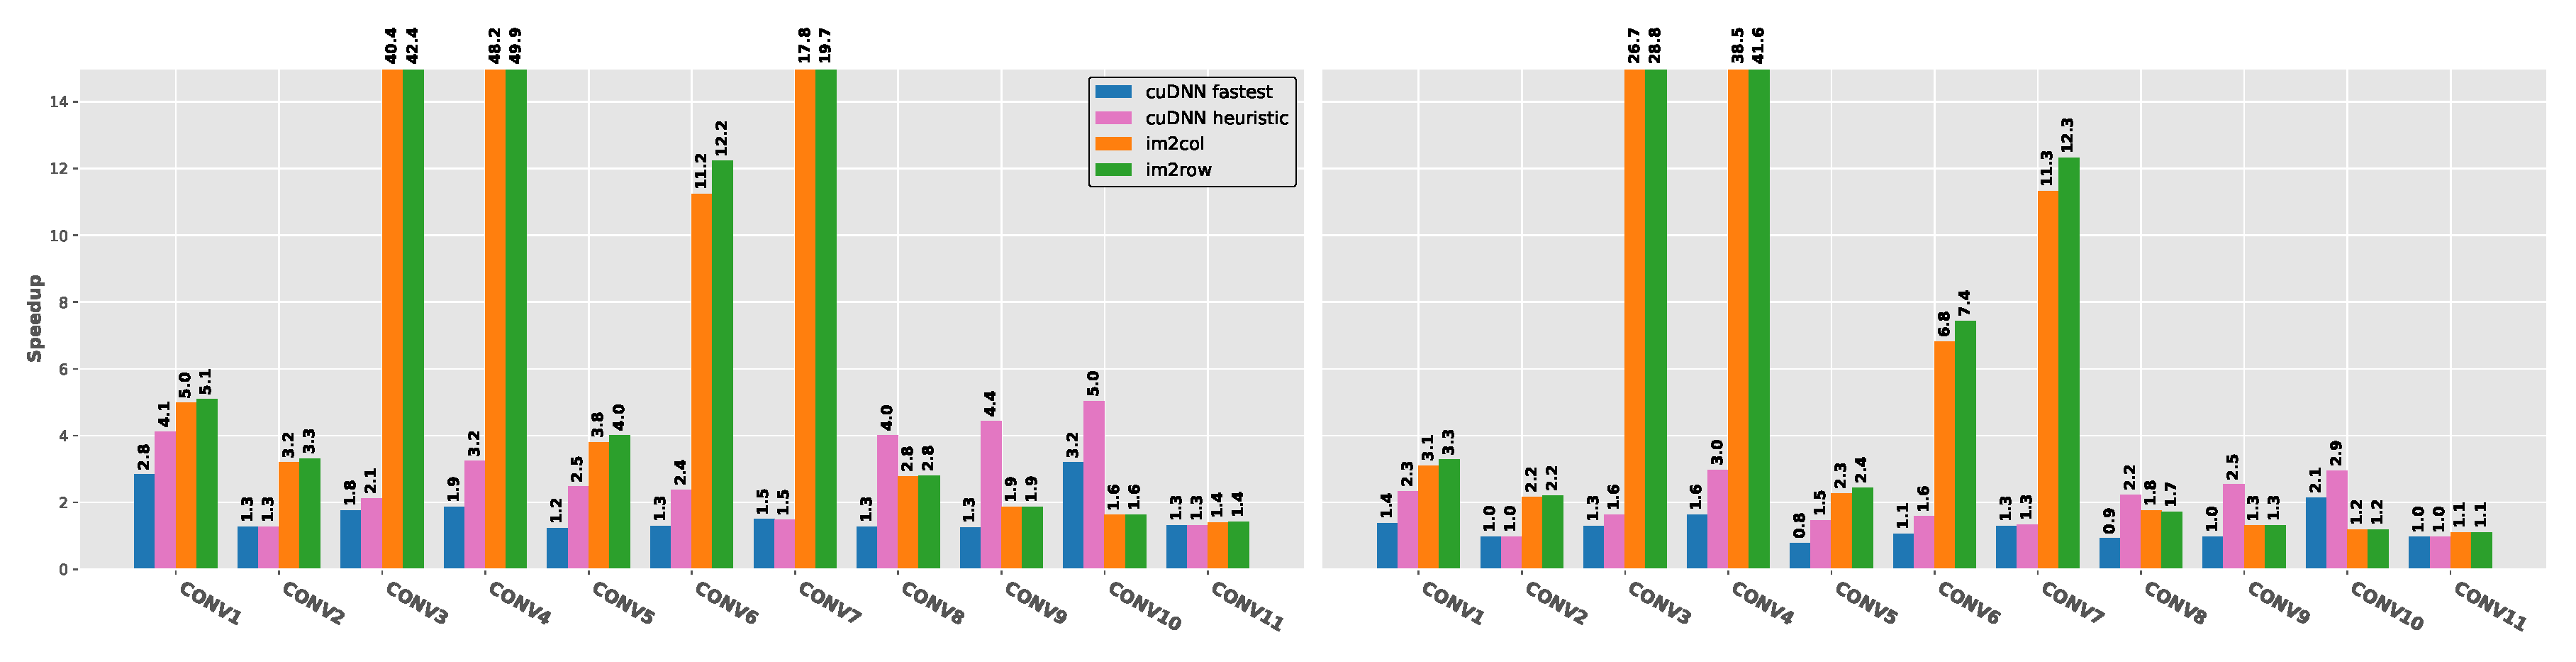
\includegraphics[width=\columnwidth,height=5cm]{./figure/3d_norm_c1.eps}
%		 \caption{Normalized runtime for convolutions with three input channels.}
%		 \label{fig:3druntimec3}
%	\end{subfigure}
%	
%	\caption{Runtime comparison among five implementations of 3D convolutions. Each runtime is normalized to our implementation.}
%   \label{fig:3druntime}
%\end{figure*}

\begin{table*}[]
\caption{The number of memory transactions for 3D convolution. Data is collected on Tesla K40m.}
\label{tab:3dtrans}
\begin{tabular}{c|ccccc|ccccc}
\hline
\multicolumn{1}{l|}{} & \multicolumn{5}{c|}{$I_C=F_C=1$}                                                                                                                                                                                                                                                                  & \multicolumn{5}{c}{$I_C=F_C=3$}                                                                                                                                                                                                                                                                  \\ \hline
    & \begin{tabular}[c]{@{}c@{}}cuDNN\\ fastest\end{tabular} & \begin{tabular}[c]{@{}c@{}}cuDNN\\ heuristic\end{tabular} & im2col & im2row & \begin{tabular}[c]{@{}c@{}}our 3D\\ conv\end{tabular} & \begin{tabular}[c]{@{}c@{}}cuDNN\\ fastest\end{tabular} & \begin{tabular}[c]{@{}c@{}}cuDNN\\ heuristic\end{tabular} & im2col & im2row & \begin{tabular}[c]{@{}c@{}}our 3D\\ conv\end{tabular} \\ \hline
CONV1& 1.7E+06& 1.2E+07& 2.3E+06& 2.3E+06& \textbf{8.5E+05}& 3.9E+06& 1.3E+07& 5.5E+06& 5.5E+06& \textbf{2.4E+06}\\
CONV2& 6.9E+06& 6.9E+06& 4.8E+06& 4.8E+06& \textbf{9.7E+05}& 1.6E+07& 1.6E+07& 1.2E+07& 1.2E+07& \textbf{2.9E+06}\\
CONV3& 3.5E+05& 1.9E+05& 1.9E+05& 2.5E+05& \textbf{8.4E+04}& 9.5E+05& 5.2E+05& 5.2E+05& 6.8E+05& \textbf{2.5E+05}\\
CONV4& 2.7E+05& 2.4E+05& 3.0E+05& 3.6E+05& \textbf{2.4E+04}& 7.4E+05& 6.4E+05& 8.0E+05& 9.8E+05& \textbf{7.3E+04}\\
CONV5& 8.7E+06& 4.5E+06& 5.1E+06& 6.5E+06& \textbf{1.4E+06}& 1.2E+07& 1.2E+07& 1.4E+07& 1.8E+07& \textbf{4.1E+06}\\
CONV6& 2.2E+06& 1.2E+06& 1.3E+06& 1.7E+06& \textbf{3.4E+05}& 5.9E+06& 3.2E+06& 3.6E+06& 4.6E+06& \textbf{1.0E+06}\\
CONV7& 1.6E+06& 1.6E+06& 1.3E+06& 1.6E+06& \textbf{1.3E+05}& 1.7E+06& 4.3E+06& 3.6E+06& 4.5E+06& \textbf{3.9E+05}\\
CONV8& 1.3E+07& 2.4E+07& 4.7E+06& 4.8E+06& \textbf{3.4E+06}& 3.0E+07& 2.9E+07& 1.1E+07& 1.2E+07& \textbf{9.8E+06}\\
CONV9& 2.7E+07& 5.5E+07& 9.9E+06& 1.0E+07& \textbf{3.9E+06}& 6.5E+07& 5.7E+07& 2.4E+07& 2.4E+07& \textbf{1.2E+07}\\
CONV10& 3.1E+07& 1.1E+08& 2.0E+07& 2.0E+07& \textbf{1.6E+07}& 7.1E+07& 1.2E+08& 5.0E+07& 5.1E+07& \textbf{4.3E+07}\\
CONV11& 1.2E+08& 1.2E+08& 7.5E+07& 7.5E+07& \textbf{2.6E+07}& 2.8E+08& 2.7E+08& 2.0E+08& 2.0E+08& \textbf{7.1E+07}\\ \hline
\end{tabular}
\end{table*}

We also apply Algorithm \ref{algo:basic}, Algorithm \ref{algo:basic2} and Algorithm \ref{algo:rowreuse} on 3D convolution. Nowadays, the most commonly used scenario of 3D convolution is CNNs. Therefore we implement a 3D convolution with one and three input channels. The main focus of this work is to optimize memory transactions not the implementation of convolution. Thus, our convolutions do not optimize on input channels. As shown in Algorithm \ref{algo:overalldesign}, our implementation is a linear scale with the number of input channels. Therefore, our implementation is more suitable for convolutions with one and three input channels, which are normally the first layers of a CNN.

We present performance comparison of 3D convolution among four implementations, including cuDNN, im2col, im2row and our implementation. We evaluate the performance of 3D convolution from three aspects, the speedup, the number of memory transactions and the memory consumption. For cuDNN, we obtain two types of runtime. First, we run all algorithms provided in cuDNN and obtain the fastest runtime, which is denoted as \emph{cuDNN fastest}. Second, we run cuDNN without specifying the algorithm, in which case cuDNN uses a heuristic method to find the most suitable algorithm for a convolution configuration. The runtime generated by the heuristic method is denoted as \emph{cuDNN heuristic}. The reason to obtain the heuristic runtime is that popular machine learning frameworks, such as Pytorch, TensorFlow and Caffe, use cuDNN with  the heuristic method in their implementations. Pythorch also uses the fastest algorithm of cuDNN in some cases.

\begin{figure*}
	
	\begin{subfigure}{\columnwidth}
		\centering
		 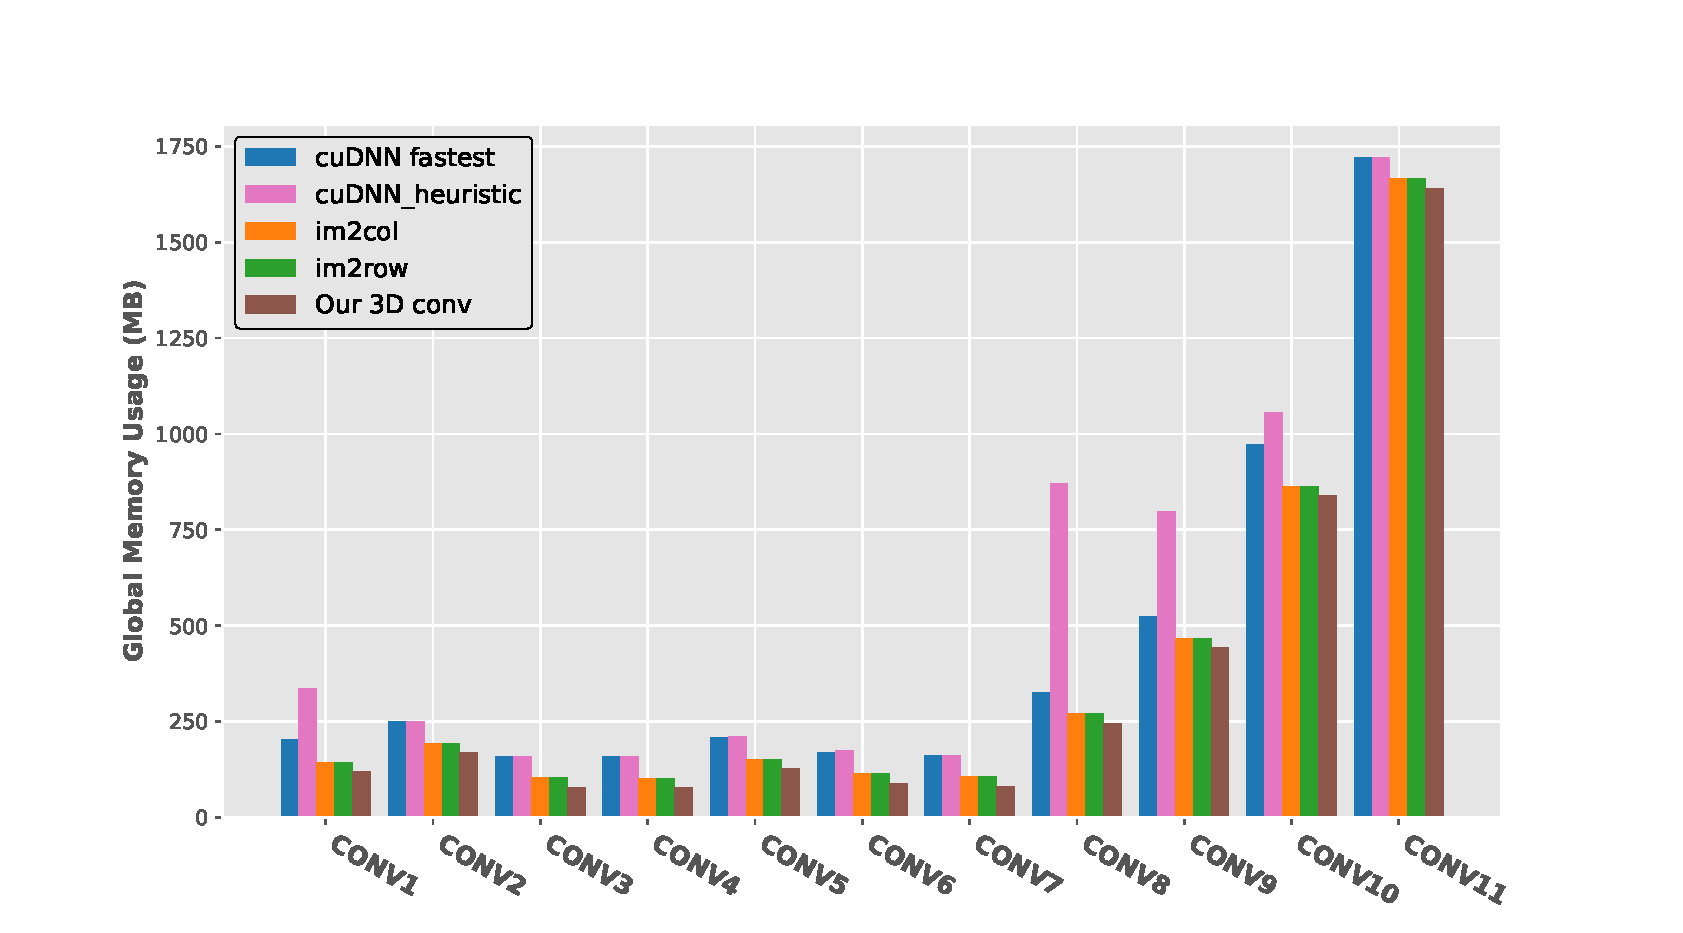
\includegraphics[width=\columnwidth,height=6cm]{./figure/mem3d_1.eps}
		 %\caption{Global memory usage for five implementations on Tesla K40m.}
		 \label{fig:3dmemk40m}
	\end{subfigure}
	\begin{subfigure}{\columnwidth}
		\centering
		 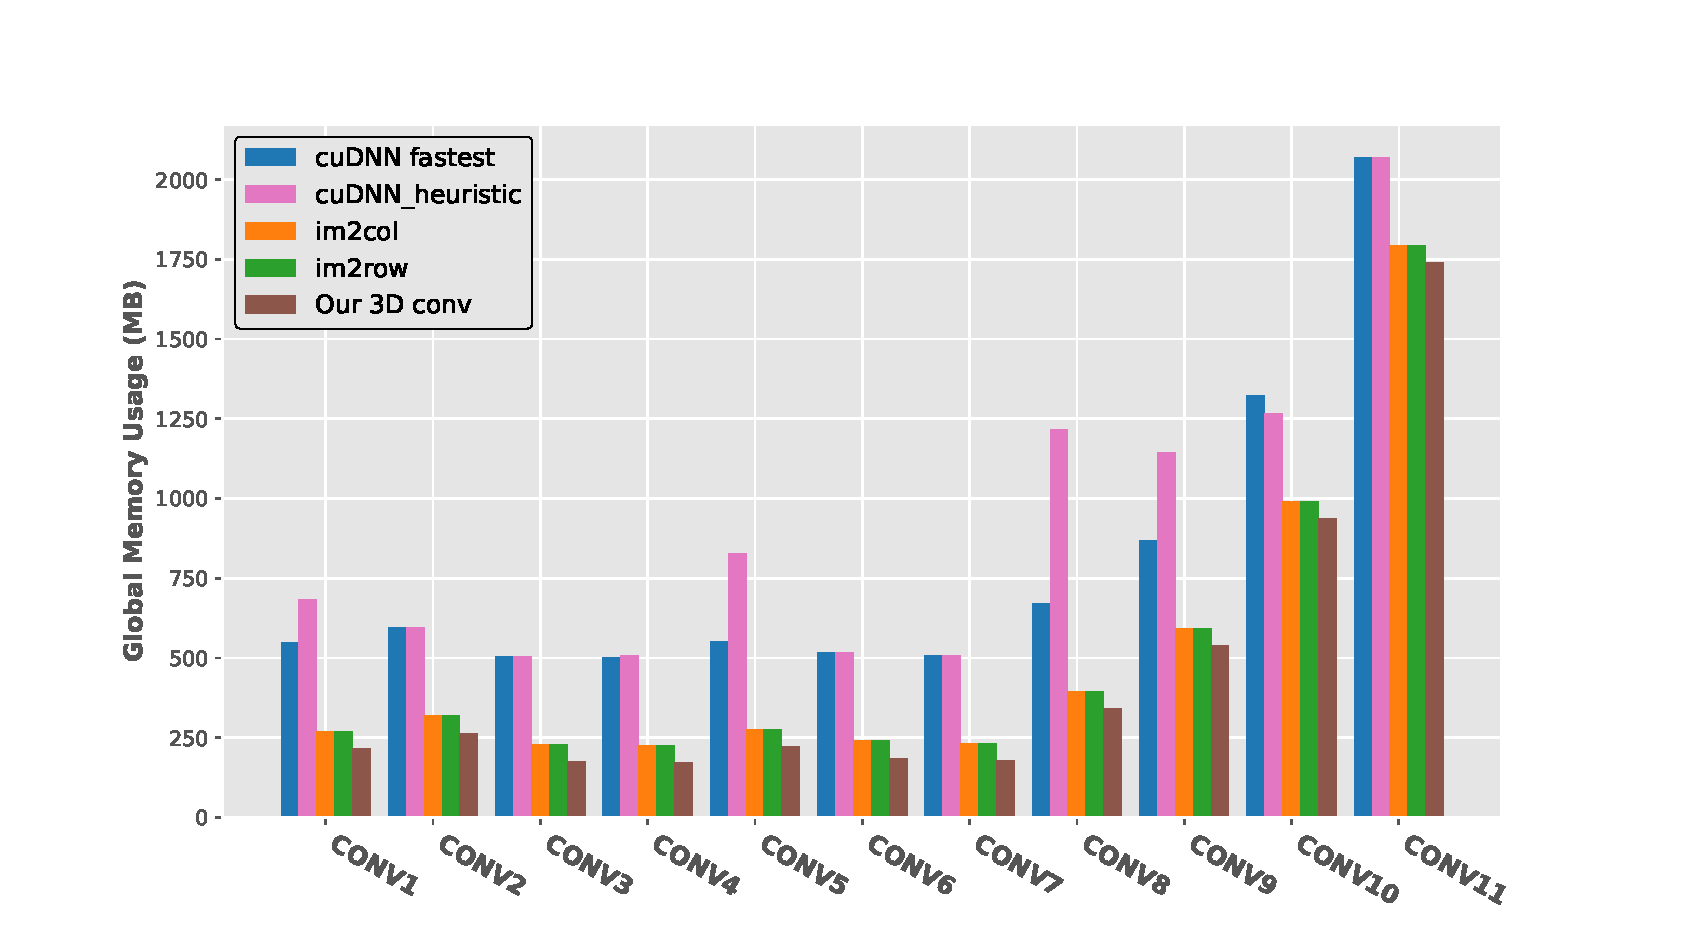
\includegraphics[width=\columnwidth,height=6cm]{./figure/mem3d_1_rtx2080.eps}
		 %\caption{Global memory usage for five implementations on RTX 2080 Ti.}
		 \label{fig:3dmemrtx2080}
	\end{subfigure}
	\caption{Global memory usage for five implementations. Left figure demonstrates the result on Tesla K40m and right figure demonstrates the result on RTX 2080 Ti.}
	\label{fig:3dmem}
\end{figure*}

We collect configurations of convolutional layers with filters of size $3 \times 3$ and $5 \times 5$ from four popular CNN models, including AlexNet \cite{Krizhevsky2012ImageNet}, VGG \cite{SimonyanZ14a}, ResNet \cite{HeZRS16} and GoogleLeNet \cite{SzegedyLJSRAEVR15}. Then we set the number of input channels to one and three ($I_C=F_C \in \{1, 3\}$) and the batch size to 128 ($I_N=O_N=128$). Other batch sizes have the similar performance because all tested implementations have a linear scale as the batch size. Exact configuration is shown in Table \ref{tab:3dconvconfigs}.

We test all 3D convolution implementations on two platforms, speedups of our implementation over the other four implementations are shown in Figure \ref{fig:3druntime}. We can see that im2col and im2row perform poorly in most cases, especially on RTX 2080 Ti. Our implementation achieves average speedups of 17.9$\times$ and 18.8$\times$ over im2col and im2row on two platforms. Figure \ref{fig:3druntimeK40} shows speedups on Tesla K40m, though cuDNN is highly optimized for 3D convolution on GPU, our implementation can still obtain an average speedup of 1.5$\times$ and 2.3$\times$ with respect to cuDNN fastest and cuDNN heuristic respecitively. Figure \ref{fig:3druntime2080} shows speedups on RTX 2080 Ti, compared with cuDNN fastest, we achieve an average speedup of 1.2$\times$ and the maximum speedup can be up to 2.5$\times$. The speedup over cuDNN heuristic is much higher, it can be 2.2$\times$ on average and the maximum speedup can be up to 6.2$\times$.

Different from 2D convolution, the performance gains of 3D convolution are obtained from two aspects, reduction on memory transactions of input data and filters. Once we load a filter into shared memory, we try to use it to slide over as many images as possible. In this way we do not need to load the same filter for each input. In Table \ref{tab:3dtrans}, we show the number of memory transactions for four implementations on Tesla K40m. We use the same method as 2D convolution to collect the number of memory transactions. Our approach achieves the minimum transaction counts in all tested cases and can averagely reduce the number of memory transactions by a factor of 6.1 and 4.4 with respect to \emph{cuDNN fastest} for one and three input channels respectively. Compared with transaction counts in 2D convolution (Table \ref{tab:2dmemtrans}), transaction counts in 3D convolution have a lower ratio with respect to other implementations. The reason is that in 3D convolution, each filter needs to slide over all inputs and thus we need to load the same filter multiple times. Though we have optimized the usage of filters, we still need to load the filters multiple times since the capacity of shared memory can not fit the whole filters. As a consequence, the number of memory transactions increases.

For 3D convolution, memory usage is also important for the scarce memory storage in GPU. We use \emph{nvidia-smi} command provided by NVIDIA CUDA Toolkit to record the peak GPU device memory usage when the application is running. We report global memory usage only for convolutions with one input channel. The reason is that output data consumes most memory storage compared with input and filter data, changing the number of input channels alone does not change the size of output data. Therefore memory usage has little change when we change the number of input channels alone.

Figure \ref{fig:3dmem} demonstrates the memory usage of four implementations on two platforms. Our implementation is derived from direct convolution which does not require extra memory, thus our implementation consumes the minimum memory storage. GEMM based implementations (im2col and im2row) first transform filters into a large matrix and then transform one input into a matrix each time they perform a matrix multiplication. Therefore, they only need extra memory to store transformed filters and one transformed input. The most memory consuming implementation is cuDNN. Since cuDNN is closed source, we could only guess that it improve the performance at a cost of memory usage. The memory consumption of our implementation is reduced by 335MB on average, 384MB  for maximum compared with cuDNN fastest. The commonly used cuDNN heuristic consumes even more memory than cuDNN fastest. Compared with cuDNN heuristic, our implementation reduces the memory consumption by 442MB on average and the maximum reduction can be up to 876MB.

In summary, our optimization algorithms successfully reduce the number of memory transactions and improve the performance of 3D convolution on two platforms. Our implementation does not need any extra memory while cuDNN consumes a large amount of memory to accelerate convolution operation, especially for cuDNN heuristic.
%From Table \ref{tab:3dspeedup} we can see that as the channel number increases, the speedup of cuDNN, im2col and im2row decrease obviously. We analyze the algorithms of im2col and im2row. Both transform the channels into a large matrix and the use the highly optimized gemm library to do the real work. When we increase the number of channels, the size of the transformed matrix also increases. But the gemm library can distribute the work among gpu cores very well, which brings little overhead on each gpu core. Though without the source code of cuDNN, we use $nvprof$ to analyze cuDNN and find that cuDNN also utilizes gemm library to do the real work. Therefore the reason also holds for cuDNN. In our implementation, we loop over each channel to calculate the final result. As the channel number increases, out implementation shows a linear scale as channel number. Therefore, as the channel number increases, the speed up of our implementation over cuDNN, im2col and im2row decreases. ArrayFire uses a similar method as our implementation, the speedup over ArrayFire is not decreased. Further optimization on channel number will be explored in the future. In this work, we mainly focus on the effectiveness of our two reuse algorithms not the implementation of the convolution.

%Second, compare through 3*3 and 5*5, we can find that for cudnn im2col im2row npp 's sppedup keep same across different filter size, but ArrayFire decreasees, the reason is that when compailing for filter 5, we have to reduce the number of each thread. or it will generate

\section{Conclusion}
In this work we propose two reuse algorithms which can significantly reduce the number of memory transactions. We use CUDA shuffle instructions to eliminate column duplications and row reuse to eliminate row duplications. To convert dynamic indexing into static indexing, we design a method with $pack$ and $unpack$ instructions provided by CUDA Toolkit. Experiments on 2D and 3D convolutions show that our reuse algorithms significantly improve the performance compared with state-of-the-art libraries. Furthermore, our implementation is derived from direct convolution, which means that we improve the performance without incurs extra memory storage.
%% Acknowledgmentsc
\begin{acks}                            %% acks environment is optional
                                        %% contents suppressed with 'anonymous'
  %% Commands \grantsponsor{<sponsorID>}{<name>}{<url>} and
  %% \grantnum[<url>]{<sponsorID>}{<number>} should be used to
  %% acknowledge financial support and will be used by metadata
  %% extraction tools.
  This material is based upon work supported by the
  \grantsponsor{GS100000001}{National Science
    Foundation}{http://dx.doi.org/10.13039/100000001} under Grant
  No.~\grantnum{GS100000001}{nnnnnnn} and Grant
  No.~\grantnum{GS100000001}{mmmmmmm}.  Any opinions, findings, and
  conclusions or recommendations expressed in this material are those
  of the author and do not necessarily reflect the views of the
  National Science Foundation.
\end{acks}


%% Bibliography
\bibliography{ref}

\end{document}
